% ======================================================================
% The Enforceability of Distinction
% Submitted to Foundations of Physics, March 2026
% ======================================================================

\documentclass[11pt]{article}

\usepackage[T1]{fontenc}
\usepackage[utf8]{inputenc}
\usepackage[a4paper,margin=1in]{geometry}
\usepackage{setspace}
\usepackage{parskip}
\usepackage{enumitem}
\usepackage{booktabs}
\usepackage{array}
\usepackage{amsmath,amssymb,amsfonts}
\usepackage{tikz}
\usepackage{mathtools}
\usepackage[most]{tcolorbox}
\usepackage{titlesec}

\titleformat{\section}{\Large\bfseries}{\thesection.}{0.5em}{}
\titleformat{\subsection}{\large\bfseries}{\thesubsection}{0.5em}{}
\titleformat{\subsubsection}{\normalsize\bfseries}{\thesubsubsection}{0.5em}{}

\pagestyle{plain}

\usepackage[colorlinks=true,linkcolor=black,citecolor=black,urlcolor=black]{hyperref}

\tcbuselibrary{skins,breakable}

\tcbset{
    apfbox/.style={
        enhanced,
        colback=black!3,
        frame hidden,
        borderline={0.5pt}{0pt}{black},
        arc=0pt,
        left=8pt, right=8pt, top=8pt, bottom=8pt,
        fonttitle=\bfseries\color{black},
        coltitle=black,
        detach title,
        before upper={\tcbtitle\par\smallskip},
        before skip=14pt,
        after skip=14pt,
        grow to left by=-8pt,
        grow to right by=-8pt,
        sharp corners,
        breakable,
    }
}

\newenvironment{varlist}{\begin{itemize}[nosep,leftmargin=2em]}{\end{itemize}}
\newcommand{\coderef}[2]{\smallskip\noindent\textit{Code reference:} \texttt{#1} in \texttt{#2}.}

\title{The Enforceability of Distinction: Finite Capacity, the Quantum Skeleton, and the Correlation Space}

\author{E.\ S.\ Brooke}

\date{}

\setstretch{1.05}
\setlist[itemize]{itemsep=3pt,topsep=4pt}
\setlist[enumerate]{itemsep=3pt,topsep=4pt}

\begin{document}
\maketitle

\noindent\textit{Independent Researcher, San Anselmo, California, USA}\\
\textit{Corresponding author: ebrooke@cleanwater1.com}\\
\textit{ORCID: https://orcid.org/0009-0001-2261-4682}

\bigskip

\begin{abstract}
\noindent
The Standard Model's 26 free parameters, three gauge groups, and three generations are inserted by hand.  This paper proposes that all such structure is \emph{forced} by a single constraint: maintaining any physical distinction---spin-up versus spin-down, here versus there, proton versus neutron---costs a share of a finite endowment.  We formalize this as Axiom~A1: enforcement capacity is finite and positive.

From A1 alone---supplemented by two definitional sub-clauses (Multiplicity, Non-Degeneracy), both subsequently derived from the framework's field content---we prove four structural lemmas: $L_{\varepsilon^*}$ (Minimum Cost), $L_{\mathrm{loc}}$ (Locality), $L_{\mathrm{nc}}$ (Non-Closure), and $L_{\mathrm{irr}}$ (Irreversibility).  An operational postulate $L_\Delta$ (Competition), derived from A1 and a perturbation model, establishes the superadditivity separating quantum structure from classical overflow.

A bridge theorem shows that superadditivity forces order-dependent enforcement---the operational content of noncommutativity---on an abstract state set without assuming Hilbert-space structure.  Standard results (Gel'fand--Na\u{\i}mark--Segal construction, Gleason's theorem, Wedderburn--Artin, Skolem--Noether) whose hypotheses are verified in each case then yield Hilbert space, the Born rule, completely positive trace-preserving dynamics, tensor products, gauge symmetry, and von Neumann entropy as committed capacity.

The framework is dimensionless: all predictions are pure numbers requiring one energy scale for unit conversion.  Twenty-three theorems with constructive witnesses and executable code references are provided.  Specific gauge groups, particle content, and the full set of zero-parameter predictions are derived in the companion papers.
\end{abstract}

\noindent\textbf{Keywords:} quantum foundations $\cdot$ finite information $\cdot$ enforcement capacity $\cdot$ quantum reconstruction $\cdot$ admissibility $\cdot$ operator algebra

\bigskip

% ======================================================================
\section{Introduction: from free parameters to forced structure}
% ======================================================================

The Standard Model of particle physics is the most precisely tested scientific theory in history.  It predicts the electron's magnetic moment to twelve decimal places, accounts for every particle observed at the Large Hadron Collider, and has survived four decades of experimental assault without a single confirmed failure.  And yet it explains almost nothing about its own structure.  Why three generations of fermions and not two or seven?  Why the gauge group $SU(3) \times SU(2) \times U(1)$ and not some other?  Why 26 free parameters with these particular values?  The Standard Model does not say.  It takes these as inputs and never looks back.

This paper proposes that the structure is not chosen but \emph{forced}---by a constraint so elementary that it has been hiding in plain sight.

\subsection{The finite universe}

What if the reason physics looks the way it does---quantum mechanics, three generations, three gauge groups, four spacetime dimensions, a cosmological constant 122 orders of magnitude below the natural scale---was never a choice, but an inevitability---forced by the single fact that the universe's resources are finite?

Start with what is least controversial.  The universe began.  Roughly 13.8 billion years ago, everything that exists emerged from a state of extraordinary compression---finite energy, finite volume, finite entropy.  It is still expanding, still cooling, still diluting.  The Big Bang was, at its core, a \emph{flow event}: a finite quantity of something---energy, degrees of freedom, information capacity---entered the arena, unfolded into structure, and produced everything we observe.  A flow event with a beginning implies a finite throughput.  A finite throughput implies a bounded total.  And yet, despite this, the idea that the universe operates under a hard \emph{capacity constraint} has received remarkably little systematic attention.  Physics has spent a century building theories on continuous symmetries, infinite-dimensional Hilbert spaces, and unbounded operator spectra---mathematical machinery that treats capacity as unlimited, even though the universe it describes plainly began with a finite endowment and will plainly end with one.

The mathematics of finite systems, by contrast, has long understood that bounded resources force structure.  Ashby's Law of Requisite Variety~\cite{Ashby1956}---the foundational theorem of cybernetics---established that a finite controller can regulate only as many distinct states as its own capacity permits.  Regulation requires resources; bounded resources limit what can be regulated; and the \emph{structure} of the controller is constrained by what it must regulate.  This principle has been applied to control theory, biology, organizational design, and information theory---but never, until now, as a foundational axiom of physics.

The primitive concept we need is the \emph{distinction}: a partition of possibilities into two classes, ``this'' and ``not this.''  Spencer-Brown's \emph{Laws of Form}~\cite{SpencerBrown1969} demonstrated that the act of drawing a distinction is the most elementary operation from which logical and algebraic structure can be generated---an insight that influenced both the theory of computation and second-order cybernetics.  In physics, distinctions are everywhere: spin-up versus spin-down, here versus there, proton versus neutron.  Each is a binary fact that the universe keeps true, moment to moment, against everything that would blur it out.

Distinctions do not exist in isolation; they are bound together by \emph{correlations}.  The spin of an electron is correlated with the magnetic field it sits in.  The polarizations of an entangled pair are correlated across arbitrary distances~\cite{Bell1964}.  A hydrogen atom is a web of correlations between the electron's quantum numbers and the proton's.  Correlations are what give structure to the physical world; without them, distinctions would be isolated labels signifying nothing.

But here is a pattern that standard physics has quantified in extraordinary detail without ever recognizing as a single phenomenon: \emph{maintaining a distinction costs something.}  A spin state is stable because an energy gap protects it---thermal fluctuations below the gap cannot flip it.  A qubit in a quantum computer stays coherent only as long as error correction actively shields it~\cite{NielsenChuang2000}.  A proton stays distinct from a neutron because QCD binding energies make the mass difference robust against perturbations.  In every case, nature commits resources to keeping a physical fact physical.  We call this commitment \textbf{enforcement}: the minimum expenditure required to maintain a distinction against all perturbations that would destroy it.

Enforcement is not observation.  It is not measurement.  It is what nature does to keep physical facts physical, whether or not anyone is looking.  Physics has quantified each instance precisely---energy gaps in electron volts, free energies in units of $kT$~\cite{Jaynes1957}, error-correction thresholds as dimensionless rates~\cite{NielsenChuang2000}, string tensions in GeV/fm~\cite{Wilson1974}, entropy bounds in bits~\cite{Bekenstein1981}---but each sub-discipline uses its own currency, its own formalism, its own units.  There is no exchange rate between them.  There is no concept of a total budget.  The Standard Model can compute the binding energy of a proton to four significant figures; what it cannot tell you is that this binding energy, the energy gap protecting a spin state, the error-correction overhead preserving a qubit, and the Bekenstein bound limiting a black hole are all denominated in the same currency---enforcement capacity---and that the sum is bounded.

Return now to the Big Bang.  If the universe began as a finite flow event, and if maintaining every physical distinction costs a share of that finite endowment, then the total number of distinctions the universe can simultaneously maintain is \emph{bounded}.  Not approximately, not in some limit, but absolutely: there is a budget, and everything must fit within it.  This is Ashby's Law applied to the universe itself: the variety of physical law is limited by the capacity of the enforcer.

This is the axiom.

\begin{center}
\textbf{A1: Enforcement capacity is finite and positive.}
\end{center}

\noindent One sentence.  No mention of quantum mechanics, gauge groups, spacetime, or particles.  Just: the cost of maintaining distinctions is bounded.  The rest of this paper shows that this single constraint---applied through standard mathematics (the GNS construction~\cite{GNS1943}, Gleason's theorem~\cite{Gleason1957}, the Wedderburn--Artin decomposition~\cite{Wedderburn1908,Artin1927}, Skolem--Noether~\cite{Skolem1927,Noether1933})---forces quantum structure, gauge symmetry, the seeds of particle content, gravitational scaling, and the thermodynamic arrow of time as necessary consequences.  Not choices.  Not parameters.  Not inputs.  Consequences.

The present paper establishes the foundation: the axiom, four structural lemmas, an operational postulate connecting finite resources to superadditivity, a bridge theorem connecting superadditivity to algebraic noncommutativity, and the structural skeleton from which the companion papers derive the Standard Model's 26 parameters, three generations, and 47 zero-parameter predictions.


\subsection{The enforcement spectrum: from easy physics to hard problems}

The ratio of enforcement demand to available capacity---$E/C$---organizes all of physics into a single spectrum (Figure~\ref{fig:spectrum}).  This ratio explains why some physics is ``easy,'' why some is ``hard,'' and why existing formalisms break down where they do.

\begin{figure}[ht]
\centering
\begin{tcolorbox}[
  enhanced,
  colback=white,
  colframe=black,
  boxrule=0.5pt,
  arc=0pt,
  left=6pt, right=6pt, top=6pt, bottom=6pt,
  sharp corners,
]
\centering
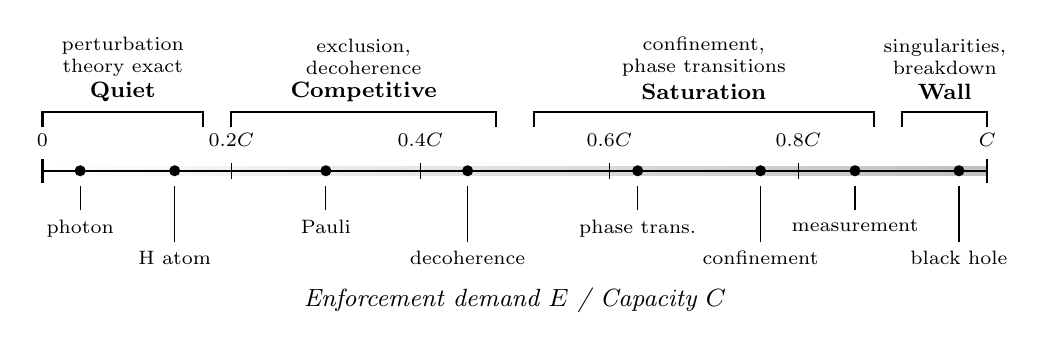
\begin{tikzpicture}[x=12cm, y=1cm]

% --- Gradient shading (behind everything) ---
\shade[left color=white, right color=black!25] (0,-0.06) rectangle (1,0.06);

% --- Main axis ---
\draw[thick] (0,0) -- (1,0);
\draw[thick] (0,-0.15) -- (0,0.15);
\draw[thick] (1,-0.15) -- (1,0.15);

% Tick marks + labels ABOVE axis
\foreach \x/\lab in {0/{0}, 0.2/{0.2$C$}, 0.4/{0.4$C$}, 0.6/{0.6$C$}, 0.8/{0.8$C$}, 1.0/{$C$}} {
  \draw (\x,-0.1) -- (\x,0.1);
  \node[above, font=\scriptsize] at (\x,0.18) {\lab};
}

% --- Regime brackets ---
\draw[thick] (0,0.55) -- (0,0.75) -- (0.17,0.75) -- (0.17,0.55);
\node[font=\footnotesize\bfseries] at (0.085,1.0) {Quiet};
\node[font=\scriptsize, text width=2cm, align=center] at (0.085,1.45) {perturbation\\theory exact};

\draw[thick] (0.20,0.55) -- (0.20,0.75) -- (0.48,0.75) -- (0.48,0.55);
\node[font=\footnotesize\bfseries] at (0.34,1.0) {Competitive};
\node[font=\scriptsize, text width=2.6cm, align=center] at (0.34,1.45) {exclusion,\\decoherence};

\draw[thick] (0.52,0.55) -- (0.52,0.75) -- (0.88,0.75) -- (0.88,0.55);
\node[font=\footnotesize\bfseries] at (0.70,1.0) {Saturation};
\node[font=\scriptsize, text width=2.6cm, align=center] at (0.70,1.45) {confinement,\\phase transitions};

\draw[thick] (0.91,0.55) -- (0.91,0.75) -- (1.0,0.75) -- (1.0,0.55);
\node[font=\footnotesize\bfseries] at (0.955,1.0) {Wall};
\node[font=\scriptsize, text width=1.6cm, align=center] at (0.955,1.45) {singularities,\\breakdown};

% --- System markers: staggered rows ---
\fill (0.04,0) circle (2pt);
\draw (0.04,-0.2) -- (0.04,-0.5);
\node[below, font=\scriptsize, anchor=north] at (0.04,-0.5) {photon};

\fill (0.30,0) circle (2pt);
\draw (0.30,-0.2) -- (0.30,-0.5);
\node[below, font=\scriptsize, anchor=north] at (0.30,-0.5) {Pauli};

\fill (0.63,0) circle (2pt);
\draw (0.63,-0.2) -- (0.63,-0.5);
\node[below, font=\scriptsize, anchor=north] at (0.63,-0.5) {phase trans.};

\fill (0.86,0) circle (2pt);
\draw (0.86,-0.2) -- (0.86,-0.5);
\node[below, font=\scriptsize, anchor=north] at (0.86,-0.5) {measurement};

\fill (0.14,0) circle (2pt);
\draw (0.14,-0.2) -- (0.14,-0.9);
\node[below, font=\scriptsize, anchor=north] at (0.14,-0.9) {H atom};

\fill (0.45,0) circle (2pt);
\draw (0.45,-0.2) -- (0.45,-0.9);
\node[below, font=\scriptsize, anchor=north] at (0.45,-0.9) {decoherence};

\fill (0.76,0) circle (2pt);
\draw (0.76,-0.2) -- (0.76,-0.9);
\node[below, font=\scriptsize, anchor=north] at (0.76,-0.9) {confinement};

\fill (0.97,0) circle (2pt);
\draw (0.97,-0.2) -- (0.97,-0.9);
\node[below, font=\scriptsize, anchor=north] at (0.97,-0.9) {black hole};

% Axis label
\node[font=\small\itshape] at (0.5,-1.65) {Enforcement demand $E$ / Capacity $C$};

% Redraw axis endpoints
\draw[thick] (0,-0.15) -- (0,0.15);
\draw[thick] (1,-0.15) -- (1,0.15);

\end{tikzpicture}

\medskip
\end{tcolorbox}
\caption{The enforcement spectrum.  Physical systems arranged by the ratio of enforcement demand to capacity ($E/C$).  Standard physics works exactly in the quiet regime, requires approximations in the competitive regime, and breaks down---singularities, the measurement problem, the information paradox---at the capacity wall.  The hard problems of physics cluster where $E/C \to 1$}
\label{fig:spectrum}
\end{figure}

\medskip\noindent\textbf{The quiet regime ($E/C \ll 1$).}
A single photon maintains two polarization states; a hydrogen atom holds a handful of quantum numbers with well-separated energy levels.  Nothing competes for resources.  Perturbation theory converges, exact solutions exist, and QED predicts the electron's anomalous magnetic moment to 12 decimal places~\cite{Aoyama2020}.  The physics is simple because the budget is barely taxed.

\medskip\noindent\textbf{The competitive regime ($E/C \sim 0.3$--$0.6$).}
The budget begins to bind.  Two electrons cannot maintain identical quantum numbers because the joint enforcement cost overflows the local budget---the Pauli exclusion principle \emph{is} non-closure.  Decoherence appears because system--environment correlations commit capacity at both interfaces, and the committed capacity is locally unrecoverable~\cite{Zurek2003}.  Perturbation theory still works but requires increasingly sophisticated approximations: the system is managing genuine competition for finite resources.

\medskip\noindent\textbf{The saturation regime ($E/C \sim 0.6$--$0.95$).}
The budget is nearly exhausted and the physics becomes dramatic.  In QCD, a free quark's unscreened color charge costs more to enforce the further it separates; when the cost exceeds interface capacity, the string snaps and produces color-singlet hadrons---fewer distinctions, lower demand~\cite{Wilson1974}.  At a phase transition, thermal perturbation costs consume the enforcement budget for the ordered state until the system can no longer afford it and transitions to disorder~\cite{Wilson1983}.  In measurement, cross-system correlations multiply as apparatus and environment entangle, saturating the budget until only one branch survives~\cite{Zurek1981}.

\medskip\noindent\textbf{The capacity wall ($E/C \to 1$).}
A black hole has saturated its enforcement capacity: $S = A/4\ell_P^2$ counts the maximum simultaneously maintainable distinctions for interface area $A$~\cite{Bekenstein1981}.  Hawking radiation is the slow release of committed capacity~\cite{Hawking1975}.  General relativity's singularity---infinite curvature, infinite density~\cite{Penrose1965}---is the formalism announcing that enforcement demand has exceeded any finite budget, which A1 forbids.  The resolution (Paper~6): curvature saturates at a finite maximum, producing a bounce rather than a singularity.

\medskip\noindent\textbf{The pattern.}  The standard formalism works beautifully in the quiet regime, requires approximations in the competitive regime, and breaks down---singularities, the measurement problem, the information paradox---at the capacity wall.  These are not separate problems.  They are the same problem: the formalism has no finite enforcement budget and cannot describe what happens when the budget runs out.  A1 supplies that concept.


\subsection{A1 is dimensionless}

A1 is dimensionless: $C$, $\varepsilon^*$, and all quantities derived from them are pure numbers.  The framework's predictions---mixing angles, mass ratios, coupling constants, $\Lambda \cdot G_N = 3\pi/102^{61}$---are dimensionless ratios.  Converting to physical units (GeV, meters, seconds) requires one dimensional input: an energy scale such as the Planck mass $M_{\mathrm{Pl}}$ or the electroweak scale $v_{\mathrm{EW}} \approx 246$~GeV.  This is a consequence of dimensional analysis (no framework can derive meters from pure mathematics), not a limitation specific to the Admissibility Physics Framework (APF).  It is the same single input the Standard Model requires.


\subsection{Context: reconstruction and finite-information programs}

This work enters a well-established tradition.  Since Hardy's seminal reconstruction of quantum theory from five operational axioms~\cite{Hardy2001}, a sustained program has sought to derive the Hilbert-space formalism from physically motivated principles rather than assume it.  Chiribella, D'Ariano, and Perinotti~\cite{CDP2011} showed that six informational axioms---including causality, distinguishability, and purification---select quantum theory uniquely from among generalized probabilistic theories.  Masanes and M\"uller~\cite{MM2011} achieved a similar result from physical requirements on state spaces and measurements.  These reconstruction programs demonstrate that ``obscure postulates'' can be replaced with principled constraints, and that the constraints themselves can be surprisingly rigid.

A1 (finite enforcement capacity) is closest in spirit to the finite-information tradition in quantum gravity.  Bekenstein's universal entropy bound~\cite{Bekenstein1981} established that bounded systems carry limited information; 't~Hooft~\cite{tHooft1993} and Susskind~\cite{Susskind1995} argued that finite degrees of freedom force holographic structure; Bousso~\cite{Bousso2002} synthesized these into the covariant entropy bound.  Jacobson~\cite{Jacobson1995} showed that Einstein's field equations emerge from thermodynamic reasoning about horizon entropy.  A1 can be read as the common ancestor of these ideas: a primitive statement that enforcement resources are finite, from which both the quantum formalism and the gravitational structure follow as consequences rather than assumptions.

What distinguishes this program from prior reconstructions is scope: where Hardy and Chiribella derive the formalism of quantum theory, the APF derives the formalism \emph{and} the specific content---gauge groups, generations, mixing angles, cosmological parameters---from a single axiom with zero free parameters.

A more precise comparison clarifies the relationship.  Chiribella, D'Ariano, and Perinotti~\cite{CDP2011} start from a well-specified mathematical setting (generalized probabilistic theories, GPTs) and impose operational axioms on that setting---purification, local tomography, causality---until quantum theory is the unique solution.  Their approach answers: \emph{given that physics is a GPT, which GPT?}  The APF answers a prior question: \emph{why should physics be a GPT at all?}  Finite enforcement capacity (A1) supplies the physical primitive that motivates finiteness of information, bounds the state space, and forces the convex-probabilistic structure that GPTs assume.  The APF does not supersede reconstruction programs; it supplies the physical grounding from which their starting point---operational structure on a bounded state space---emerges as a derived consequence rather than an axiom.  The two programs are complementary: operational axiom schemes characterize quantum theory from within a fixed setting; A1 explains why physics lives in that setting.


\subsection{The APF engine: code as specification}

Every theorem in this paper series is implemented as an executable check function in the APF codebase---a modular Python package organized by derivation layer (\texttt{core}, \texttt{gauge}, \texttt{generations}, \texttt{spacetime}, \texttt{gravity}, \texttt{cosmology}).  Each check function encodes the theorem's statement, verifies its numerical content against exact arithmetic (using Python's \texttt{Fraction} type), records its dependencies, and returns a structured result.  A separate validation module compares derived predictions to experimental benchmarks (Planck 2018~\cite{Planck2018}, PDG 2024~\cite{PDG2024}, NuFit 6.0~\cite{NuFit2024}) behind a firewall that isolates empirical data from the derivation chain.  Code references of the form \texttt{(check\_X, module.py)} appear throughout Papers 1--7.


\subsection{Road map: from axiom to physics}

This paper establishes the axiom and derives four foundational lemmas plus one operational postulate.  The derivation order is strict and acyclic:

\begin{center}
\begin{tabular}{lllll}
\toprule
\textbf{Order} & \textbf{Result} & \textbf{Type} & \textbf{Dependencies} & \textbf{Used by} \\
\midrule
1 & $L_{\varepsilon^*}$ (Minimum Cost) & Lemma & A1 & all below \\
2 & $L_{\mathrm{loc}}$ (Locality) & Lemma & A1, $L_{\varepsilon^*}$, M, NT & $L_{\mathrm{irr}}$, Papers 2--7 \\
3 & $L_{\mathrm{nc}}$ (Non-Closure) & Lemma & A1, $L_{\varepsilon^*}$, M & $L_{\mathrm{irr}}$, T1 \\
4 & $L_{\Delta}$ (Competition) & Postulate & A1, Pert.\ Model & T1, $L_{\mathrm{irr}}$ \\
5 & $L_{\mathrm{irr}}$ (Irreversibility) & Lemma & $L_{\mathrm{nc}}$, $L_\Delta$, $L_{\mathrm{loc}}$ & Papers 3, 4, 5 \\
\bottomrule
\end{tabular}
\end{center}

These feed into a bridge theorem (T1: Order-Dependence $\to$ Noncommutativity), which opens the door to the quantum skeleton (T2--$T_{\mathrm{canonical}}$) via standard mathematical results.

% ======================================================================
\section{The axiom: finite enforcement capacity}
% ======================================================================

The entire framework rests on a single physical claim.  A1 says that nature's capacity to enforce distinctions is finite and positive---nothing more.

\begin{tcolorbox}[apfbox, title={Axiom A1 (Finite Enforcement Capacity)}]
For any admissible state $\sigma$ on a causally connected region $R$,
\begin{equation}
\sum_{d \,\in\, \mathcal{D}(\sigma,\,R)} \varepsilon(d) \;\le\; C(R) \;<\; \infty
\end{equation}

\smallskip\noindent\textbf{\textit{Variables:}}
\begin{varlist}
\item $\Omega$ --- the abstract state set: the collection of all possible configurations of enforced distinctions.  No algebraic or topological structure is assumed on $\Omega$ at this stage.
\item $\sigma \in \Omega$ --- a state (a particular configuration of enforced distinctions on region $R$).
\item $R$ --- a causally connected region of the universe.
\item $\mathcal{D}(\sigma,R)$ --- the set of independently enforceable distinctions maintained in state $\sigma$ on region $R$.  Each element is a distinct physical difference that the universe actively enforces.
\item $\varepsilon(d)$ --- the enforcement cost of distinction $d$: the capacity committed to maintaining $d$ against collapse.  Bounded below: $\varepsilon(d) \ge \varepsilon^* > 0$ for all meaningful $d$.
\item $\varepsilon^*$ --- the minimum enforcement cost per distinction, strictly positive.  The framework requires $\varepsilon^* > 0$ but never requires its numerical value; all downstream results depend only on finiteness and positivity.
\item $C(R)$ --- the total enforcement capacity of region $R$: the finite upper bound on how much enforcement can be simultaneously committed within $R$.
\end{varlist}

\coderef{check\_A1}{core.py}
\end{tcolorbox}

This is a constraint on what nature can do, not on what we can observe.  The specific value of $C$ is never required; only finiteness and positivity matter.

\subsection{What A1 is not: no choices, no specifics}

A1 does not say how large $C$ is.  It does not say what the distinctions are made of.  It does not say whether the universe is classical or quantum, continuous or discrete, four-dimensional or otherwise.  All of those properties are derived in Sections 4--6 as consequences of the axiom, not written into it.

The axiom is not a simplifying assumption.  If enforcement resources are unlimited, there is no cap on how many distinctions can be maintained.  If there is no cap, then every conceivable pattern can persist---nothing is forced to give way.  If nothing is forced, there are no constraints.  And if there are no constraints, there is no physics: no selection, no structure, no law.  Finite enforceability is the minimum condition for physical law to exist.

\subsection{Sub-clauses and their derivation: M, NT, and closure}

Two definitional sub-clauses accompany A1, specifying that the universe under discussion has enough structure to be interesting.  Think of them the way one thinks of the axiom of infinity in set theory: they carry no predictive content beyond a definitional role.

\begin{tcolorbox}[apfbox, title={Sub-Clauses M (Multiplicity) and NT (Non-Degeneracy)}]
\textbf{\textit{Sub-clause M}} (Multiplicity): At least two distinguishable subsystems exist: $|\mathcal{D}| \ge 2$.

\smallskip
\textbf{\textit{Sub-clause NT}} (Non-Degeneracy): Not all subsystems are identical.  There exist subsystems $S_i, S_j$ with $C(S_i) \ne C(S_j)$.

\smallskip
Without M, the axiom is trivially satisfied by a single point with capacity $C$---no physics emerges because there is nothing to distinguish.  Without NT, every subsystem has capacity $C/N$ and no asymmetry develops---no gauge group selection, no generations, no symmetry breaking.

\coderef{check\_M, check\_NT}{core.py}
\end{tcolorbox}

Both sub-clauses are subsequently \emph{derived} from the framework's own field content.  This closes the logical loop: M and NT are assumed at the axiom layer, then proved to follow from structures that the axiom generates.  The logical status is self-consistency, not circularity---the derivation chain is acyclic (A1 $\to$ lemmas $\to$ gauge content $\to$ M, NT), and the sub-clauses are used only in the initial derivation of $L_{\mathrm{loc}}$ (Locality).  The derivations ($L_{M,\mathrm{derived}}$ and $L_{NT,\mathrm{derived}}$) are given in Appendix~C.


% ======================================================================
\section{Definitions: the language of enforcement}
\label{sec:defs}
% ======================================================================

Before deriving consequences from A1, we fix the five primitive concepts that the framework uses.  All are defined operationally in terms of enforcement on the abstract state set $\Omega$, not on a Hilbert space.  The Hilbert-space representation is \emph{derived} in Section~5.

\begin{tcolorbox}[apfbox, title={Definitions (Distinction, Enforcement Cost, Interface, Admissible State, Capacity)}]
\textbf{\textit{Distinction.}} A binary predicate $d: \Omega \to \{0, 1\}$ that partitions the state set into two non-empty subsets.  Each distinction is a physical fact the universe actively maintains: spin-up rather than spin-down, this particle here rather than there, proton rather than neutron.  A distinction is \emph{enforceable} if it is \emph{robust}: no admissible perturbation of cost less than $\varepsilon(d)$ can destroy it.

\smallskip\noindent\textbf{\textit{Variables:}}
\begin{varlist}
\item $\Omega$ --- the abstract state set.  No algebraic, topological, or linear structure is assumed.  $\Omega$ is the pre-geometric arena on which all other structures are built.
\item $d: \Omega \to \{0,1\}$ --- a distinction.  Think of $d$ as a ``yes/no'' physical fact that the universe maintains.
\item \textit{Robustness} --- a distinction $d$ is robust (hence enforceable) iff $\varepsilon(d) > 0$: there exists a minimum perturbation cost below which $d$ cannot be destroyed.
\end{varlist}

\medskip
\textbf{\textit{Enforcement Cost.}} The minimum cost of destroying a distinction $d$:
\[
\varepsilon(d) \;=\; \inf\bigl\{\mathrm{cost}(p) : p \text{ is an admissible perturbation that destroys } d\bigr\}.
\]
A distinction is \emph{robust} (hence enforceable) iff $\varepsilon(d) > 0$: every perturbation capable of destroying $d$ costs at least $\varepsilon(d)$.

\medskip
\textbf{\textit{Interface.}} A locus $\Gamma$ at which enforcement occurs.  Each interface has a capacity budget $C(\Gamma) > 0$ and enforces a subset of the total distinctions.

\medskip
\textbf{\textit{Admissible State.}} A state $\sigma \in \Omega$ is admissible if the total enforcement cost of all simultaneously maintained distinctions does not exceed the available capacity:
\[
\sum_{d \in \mathcal{D}(\sigma, R)} \varepsilon(d) \;\le\; C(R).
\]

\medskip
\textbf{\textit{Enforcement Capacity.}} $C(R)$ is the total enforcement capacity on region $R$.  It decomposes over interfaces: $C(R) = \sum_{\Gamma \in R} C(\Gamma)$.  The global capacity $C_{\mathrm{total}}$ counts the total number of distinguishable capacity types.

\medskip
\textbf{\textit{Cost-Discreteness.}}  The distinction space $\mathcal{D}$ is \emph{cost-discrete}: for any $K > 0$, the set $\{d \in \mathcal{D} : \varepsilon(d) \le K\}$ is finite.  Operationally, this says that in a universe with finite total capacity $C$, only finitely many independent physical differences can be maintained below any given energy threshold---a universe with infinitely many sub-threshold distinctions would require infinite capacity to survey, violating A1.  Cost-discreteness is not an independent physics axiom; it is a structural consequence of requiring that distinctions be individually enforceable against a bounded budget.

\medskip
\textbf{\textit{Perturbation Model.}} Perturbations targeting distinct distinctions can combine.  The perturbation space for jointly-enforced distinctions $\{d_1, d_2\}$ contains combined attacks---perturbations that simultaneously threaten both $d_1$ and $d_2$---not merely perturbations targeting each individually.  Formally: if $\mathcal{P}(d_i)$ is the set of perturbations threatening $d_i$, then the perturbation space for the joint enforcement of $\{d_1, d_2\}$ satisfies $\mathcal{P}(\{d_1, d_2\}) \supseteq \mathcal{P}(d_1) \cup \mathcal{P}(d_2)$, with the inclusion strict whenever $d_1$ and $d_2$ share enforcement resources.  Two further properties hold for resource-sharing distinctions.
\begin{itemize}[nosep,leftmargin=2em]
  \item \textit{Combined-attack efficiency}: a combined attack $p^* \in \mathcal{P}(\{d_1,d_2\}) \setminus (\mathcal{P}(d_1) \cup \mathcal{P}(d_2))$ exploits the shared budget by simultaneously degrading both distinctions at a cost strictly less than the sum of the individual minimum attack costs: $\mathrm{cost}(p^*) < \varepsilon(d_1) + \varepsilon(d_2)$.  This is the adversarial mirror of resource-sharing: attacking both distinctions through their common pool is cheaper than attacking each independently.
  \item \textit{Strict cost monotonicity}: the minimum defense cost is strictly monotone in the perturbation set.  If $\mathcal{P}' \supsetneq \mathcal{P}$, then $\min_{\text{defense defeats }\mathcal{P}'}\mathrm{cost} > \min_{\text{defense defeats }\mathcal{P}}\mathrm{cost}$, because any defense that defeats $\mathcal{P}$ does not defeat attacks in $\mathcal{P}' \setminus \mathcal{P}$, and any attack has $\mathrm{cost}(p) > 0$.
\end{itemize}
The perturbation model as a whole is mathematical infrastructure (a regularity condition on the enforcement cost functional), not a separate physics axiom; it carries the same logical status as the specification that $\Omega$ is a set or that $d$ is a binary predicate.
\end{tcolorbox}


% ======================================================================
\section{The four lemmas and the competition postulate}
\label{sec:lemmas}
% ======================================================================

The derivation chain from A1 to the full framework passes through four structural lemmas and one operational postulate ($L_\Delta$, derived from the perturbation model in Section~\ref{sec:defs}).  The derivation order is strict and acyclic:
\begin{multline*}
L_{\varepsilon^*}\;\text{(A1)} \;\to\; L_{\mathrm{loc}}\;\text{(A1 + $L_{\varepsilon^*}$ + M + NT)} \;\to\; L_{\mathrm{nc}}\;\text{(A1 + $L_{\varepsilon^*}$ + M)} \\
\to\; L_{\Delta}\;\text{(A1 + Pert.\ Model)} \;\to\; L_{\mathrm{irr}}\;\text{($L_{\mathrm{nc}}$ + $L_\Delta$ + $L_{\mathrm{loc}}$)}
\end{multline*}

Note: $L_{\mathrm{loc}}$ (Locality) and $L_{\mathrm{nc}}$ (Non-Closure) are logically independent---neither requires the other.  Both require $L_{\varepsilon^*}$.  They are ordered here to match the derivation logic: locality establishes the interface structure, then non-closure establishes that interfaces overflow.  $L_\Delta$ (Competition) connects non-closure to superadditivity via the perturbation model.


\subsection{\texorpdfstring{$L_{\varepsilon^*}$}{L epsilon*} (Minimum Cost): no infinitesimal distinctions}
\label{sec:eps_star}

If distinctions could be maintained at arbitrarily small cost, an unbounded number of them could fit within any finite capacity---and finiteness would carry no structural force.

\begin{tcolorbox}[apfbox, title={Lemma $L_{\varepsilon^*}$ (Minimum Cost)}]
\textbf{Statement.}  There exists $\varepsilon^* > 0$ such that every enforceable distinction costs at least $\varepsilon^*$:
\begin{equation}
\varepsilon(d) \;\ge\; \varepsilon^* \;>\; 0 \qquad \forall\; d \in \mathcal{D}.
\end{equation}

\smallskip\noindent\textbf{\textit{Variables:}}
\begin{varlist}
\item $\varepsilon(d)$ --- enforcement cost of distinction $d$ (Section~\ref{sec:defs}).
\item $\varepsilon^* = \inf_{d \in \mathcal{D}} \varepsilon(d)$ --- the infimum of enforcement costs over all enforceable distinctions.
\item $C$ --- total enforcement capacity (from A1).
\item \textit{Robustness} --- a distinction is enforceable iff $\varepsilon(d) > 0$: every destroyer costs at least $\varepsilon(d)$ (Section~\ref{sec:defs}).
\end{varlist}

\smallskip\noindent\textbf{Proof} (direct, using robustness and cost-discreteness).

\textit{Step 1} (Per-distinction positivity).  By the robustness definition (Section~\ref{sec:defs}), every enforceable distinction satisfies $\varepsilon(d) > 0$.  That is: for each $d \in \mathcal{D}$ individually, the enforcement cost is strictly positive.

\textit{Step 2} (Global infimum is achieved).  By cost-discreteness (Section~\ref{sec:defs}), for any $K > 0$ the set $\{d \in \mathcal{D} : \varepsilon(d) \le K\}$ is finite.  Let $\varepsilon^* = \inf_{d \in \mathcal{D}} \varepsilon(d)$.  If $\varepsilon^* > 0$, take $K = \varepsilon^*$: the set $\{d : \varepsilon(d) \le \varepsilon^*\}$ is finite and non-empty (since infimum is approached), so $\varepsilon^*$ is achieved at some $d^* \in \mathcal{D}$.  If $\varepsilon^* = 0$, then for every $n \in \mathbb{N}$ the set $\{d : \varepsilon(d) \le 1/n\}$ is finite but non-empty, which yields a sequence of distinct distinctions $d_n$ with $\varepsilon(d_n) \to 0$.  But each $d_n$ is enforceable, hence robust ($\varepsilon(d_n) > 0$), contradicting $\varepsilon(d_n) \to 0$ together with the requirement (from A1 and cost-discreteness) that no infinite descending sequence of costs can fit within the finite capacity $C$.  (Formally: infinitely many distinctions with costs $< 1/n$ for all $n$ would require infinite capacity to enumerate as enforced, contradicting $C < \infty$.)  Therefore $\varepsilon^* = 0$ is impossible, and the infimum is achieved at a strictly positive value.

\textit{Step 3} (Strict positivity).  Since $\varepsilon^*$ is achieved at $d^*$ and $\varepsilon(d^*) > 0$ by Step~1, we conclude $\varepsilon^* > 0$.

\smallskip\noindent\textbf{Conclusion.}  $\varepsilon^* > 0$.  The maximum number of simultaneously enforceable distinctions is therefore bounded:
\begin{equation}
|\mathcal{D}| \;\le\; \left\lfloor \frac{C}{\varepsilon^*} \right\rfloor \;<\; \infty.
\end{equation}

\smallskip\noindent\textbf{\textit{Key premise:}} ``meaningful = robust under admissible perturbation'' is definitional within the framework (Section~\ref{sec:defs}).  This identification is the framework's definition of physical meaningfulness; it is not an additional postulate, but it is the assumption on which $L_{\varepsilon^*}$ rests.

\coderef{check\_L\_epsilon\_star}{core.py}
\end{tcolorbox}


\subsection{\texorpdfstring{$L_{\mathrm{loc}}$}{L loc} (Locality): enforcement must distribute}

Finite capacity with enough physical structure forces enforcement to split over multiple independent interfaces.  The argument requires only $L_{\varepsilon^*}$ (for the counting bound) plus the richness conditions M and NT.  It does \emph{not} require non-closure.

\begin{tcolorbox}[apfbox, title={Lemma $L_{\mathrm{loc}}$ (Locality)}]
\textbf{Statement.}  A1 + $L_{\varepsilon^*}$ (Minimum Cost) + M + NT $\implies$ enforcement decomposes over independent interfaces.

\smallskip\noindent\textbf{\textit{Variables:}}
\begin{varlist}
\item $\Gamma$ --- an interface (enforcement locus) with capacity budget $C(\Gamma)$.
\item $n_{\max}(\Gamma) = \lfloor C(\Gamma) / \varepsilon^* \rfloor$ --- maximum distinctions enforceable at a single interface.
\item $N_{\mathrm{phys}}$ --- total number of independently meaningful distinctions.
\item \textit{Independent interfaces} --- two interfaces $\Gamma_1, \Gamma_2$ are independent iff: (i) each has its own capacity budget ($C(\Gamma_1), C(\Gamma_2)$ allocated separately); (ii) an operation at $\Gamma_1$ cannot modify the enforcement state at $\Gamma_2$ without consuming additional capacity; (iii) budget accounting at each is self-contained.  \emph{Any} partitioning of a single budget into sub-budgets satisfying (i)--(iii) constitutes independent interfaces---the distinction between ``one locus with internal partitions'' and ``multiple loci'' is definitional, not physical.
\end{varlist}

\smallskip\noindent\textbf{Proof} (four steps).

\textit{Step 1} (Single-interface capacity bound).  By A1, $C < \infty$.  By $L_{\varepsilon^*}$, each distinction costs $\ge \varepsilon^* > 0$.  A single interface can enforce at most $\lfloor C / \varepsilon^* \rfloor$ distinctions.

\textit{Step 2} (Richness exceeds single-interface capacity).  By M + NT, the number of independently meaningful distinctions $N_{\mathrm{phys}}$ exceeds any single interface's capacity: $N_{\mathrm{phys}} > \lfloor C_{\max} / \varepsilon^* \rfloor$.

\textit{Step 3} (Distribution is forced).  Since $N_{\mathrm{phys}}$ exceeds the single-interface bound, the universe must partition enforcement into sub-budgets $C_1, \ldots, C_k$ with $\sum_j C_j = C_{\mathrm{total}}$, each handling a subset of distinctions.  Coordination between sub-budgets itself requires enforcement (transferring capacity from $C_1$ to $C_2$ means modifying both enforcement states, costing $\ge \varepsilon^*$ by $L_{\varepsilon^*}$).  Under A1, unlimited coordination would consume the entire budget.  Concretely: maintaining global coherence across $k$ sub-budgets requires at least $\binom{k}{2}\varepsilon^*$ coordination cost, which for large $k$ overwhelms $C_{\mathrm{total}}$ and leaves nothing for the distinctions themselves.  The budget itself enforces the separation.  Therefore the sub-budgets are operationally independent.

\textit{Step 4} (Independence = locality).  Independent interfaces with separate budgets means: (a) no interface has global access (each enforces a proper subset); (b) enforcement decomposes: $E_{\mathrm{total}} = \sum_i E(\Gamma_i)$; (c) subsystems at disjoint interfaces are independently enforceable.  This is locality.

\smallskip\noindent\textbf{Constructive witness.}  Six distinctions with $\varepsilon = 2$ and $C = 10$:
\begin{align}
\text{Single interface:}\quad E_{\mathrm{full}} &= \tfrac{39}{2} = 19.5 > 10 = C \quad\text{(inadmissible)} \\
\text{Two interfaces:}\quad E_{\mathrm{left}} = E_{\mathrm{right}} &= \tfrac{33}{4} = 8.25 \le 10 = C \quad\text{(admissible)}
\end{align}

\smallskip\noindent\textbf{Countermodel.}  $|\mathcal{D}| = 1$: a single interface with $C \ge \varepsilon^*$ suffices.  Confirms M is necessary.

\coderef{check\_L\_loc}{core.py}
\end{tcolorbox}


\subsection{\texorpdfstring{$L_{\mathrm{nc}}$}{L nc} (Non-Closure): composition overflows capacity}

Non-closure is the engine behind competition, saturation, and selection.  It requires only finite capacity and positive costs---no spatial structure or locality is needed.  $L_{\mathrm{nc}}$ and $L_{\mathrm{loc}}$ are logically independent: each depends on $L_{\varepsilon^*}$, but neither depends on the other.

The idea is immediate from a concrete example.  Suppose the total enforcement budget is $C = 10$.  Sector~$S_1$ (say, a collection of color-charge distinctions) costs $E_1 = 6$ to enforce; sector~$S_2$ (say, a collection of electroweak distinctions) also costs $E_2 = 6$.  Each sector is individually admissible: $6 \le 10$.  But their composition demands $E_1 + E_2 = 12 > 10$---the budget overflows.  The universe cannot afford both at full strength simultaneously.  Something must give: one sector is suppressed, resources are redistributed, or new structure emerges to manage the competition.  This is non-closure.

\begin{tcolorbox}[apfbox, title={Lemma $L_{\mathrm{nc}}$ (Non-Closure)}]
\textbf{Statement.}  A1 + $L_{\varepsilon^*}$ (Minimum Cost) + M $\implies$ the set of admissible states is not closed under composition.

\smallskip\noindent\textbf{\textit{Variables:}}
\begin{varlist}
\item $C$ --- total capacity budget (from A1).
\item $E_i$ --- enforcement demand of sector $i$: the total cost of enforcing all of sector $i$'s distinctions.
\item $\Omega_{\mathrm{adm}} = \{\sigma \in \Omega : \sum_d \varepsilon(d) \le C\}$ --- the set of admissible states.
\end{varlist}

\smallskip\noindent\textbf{Proof} (constructive).

\textit{Step 1} (Existence of competing sectors).  By M, at least two distinguishable sectors exist.  By $L_{\varepsilon^*}$ (Minimum Cost), each sector costs $\ge \varepsilon^* > 0$.  Therefore there exist sectors $S_1, S_2$ with $E_1, E_2 > 0$.

\textit{Step 2} (Witness).  Let $C = 10$.  Let $E_1 = 6$ and $E_2 = 6$.  Each is individually admissible:
\begin{equation}
E_1 = 6 \le 10 = C, \qquad E_2 = 6 \le 10 = C.
\end{equation}
Their composition has total demand:
\begin{equation}
E_1 + E_2 = 12 > 10 = C \qquad \text{(inadmissible)}.
\end{equation}

\textit{Step 3} (Generalization).  For any $n$ sectors each with $E_i > C/n$:
\begin{equation}
\sum_{i=1}^{n} E_i \;>\; n \cdot \frac{C}{n} \;=\; C.
\end{equation}
Such sectors exist whenever M holds (multiple subsystems) and $L_{\varepsilon^*}$ holds (each costs $> 0$).  $L_{\varepsilon^*}$ also blocks subadditive evasion: no cost function satisfying $\varepsilon(d) \ge \varepsilon^* > 0$ can make the sum converge below $C$ for arbitrarily many sectors.

\smallskip\noindent\textbf{Conclusion.}  $\Omega_{\mathrm{adm}}$ is not closed under composition.  Note that this is a purely arithmetic consequence of finite capacity and positive costs---a classical ``knapsack'' overflow.  It does \emph{not} by itself imply superadditivity ($\Delta > 0$) or interference; those require the additional structure established in $L_\Delta$ below.

\coderef{check\_L\_nc}{core.py}
\end{tcolorbox}


\subsection{\texorpdfstring{$L_{\Delta}$}{L Delta} (Competition): superadditivity from combined perturbations}

Pause here and take stock.  $L_{\mathrm{nc}}$ says that two individually affordable collections of distinctions can be jointly unaffordable---a finite budget overflows when you try to maintain everything at once.  This is a real constraint, but it is entirely classical: a shipping container has finite volume, and two loads that each fit individually may not fit together.  Nothing about non-closure, by itself, produces interference, noncommutativity, or any distinctively quantum phenomenon.  Classical budget overflow gives you a knapsack problem.  It does not give you quantum mechanics.

The passage from ``finite budget'' to ``noncommutativity'' requires something stronger: that jointly enforcing two distinctions costs \emph{strictly more} than the sum of individual costs---that is, superadditivity.  The additional cost arises because shared resources create new vulnerabilities: perturbations that could not threaten either distinction alone can threaten both when they draw on the same pool.  This is derived from A1 and the perturbation model (Section~\ref{sec:defs}).

\begin{tcolorbox}[apfbox, title={$L_{\Delta}$ (Competition): Superadditivity from Shared Budgets}]
\textbf{Statement.}  A1 + Perturbation Model $\implies$ for distinctions $d_1, d_2$ sharing an enforcement budget, the joint enforcement cost is superadditive:
\begin{equation}
\varepsilon(\{d_1, d_2\}) \;\ge\; \varepsilon(d_1) + \varepsilon(d_2) + \Delta(d_1, d_2), \qquad \Delta(d_1, d_2) > 0.
\end{equation}

\smallskip\noindent\textbf{\textit{Variables:}}
\begin{varlist}
\item $\varepsilon(\{d_1, d_2\})$ --- the joint enforcement cost: the minimum cost of maintaining \emph{both} $d_1$ and $d_2$ simultaneously against all admissible perturbations, including combined attacks.
\item $\Delta(d_1, d_2)$ --- the superadditivity surplus: the additional cost of defending against combined perturbations beyond the sum of individual defenses.
\item $\mathcal{P}(\{d_1, d_2\})$ --- the joint perturbation space, which by the Perturbation Model strictly contains $\mathcal{P}(d_1) \cup \mathcal{P}(d_2)$ for resource-sharing distinctions.
\end{varlist}

\smallskip\noindent\textbf{Proof} (geometric).

\textit{Step 1} (Individual defense).  Enforcing $d_1$ alone requires defending against perturbations in $\mathcal{P}(d_1)$ at cost $\varepsilon(d_1)$.  Likewise $d_2$ alone at cost $\varepsilon(d_2)$.

\textit{Step 2} (Joint defense must cover combined attacks).  By the Perturbation Model, the joint perturbation space $\mathcal{P}(\{d_1, d_2\})$ strictly contains $\mathcal{P}(d_1) \cup \mathcal{P}(d_2)$: there exist combined attacks $p^* \in \mathcal{P}(\{d_1, d_2\}) \setminus (\mathcal{P}(d_1) \cup \mathcal{P}(d_2))$ that target both distinctions through their shared resource.  The individual defenses (total cost $\varepsilon(d_1) + \varepsilon(d_2)$) are optimized to defeat $\mathcal{P}(d_1) \cup \mathcal{P}(d_2)$ but leave $p^*$ undefeated.

\textit{Step 2b} (Strict superadditivity via minimax).  By strict cost monotonicity (Perturbation Model), any defense that defeats the strictly larger set $\mathcal{P}(\{d_1,d_2\})$ costs strictly more than the best defense against $\mathcal{P}(d_1) \cup \mathcal{P}(d_2)$.  Formally:
\begin{equation}
\varepsilon(\{d_1,d_2\}) \;=\; \min_{\text{defense}} \max_{p \,\in\, \mathcal{P}(\{d_1,d_2\})} [\text{defense fails against } p]
\end{equation}
exceeds $\varepsilon(d_1) + \varepsilon(d_2)$ by a gap $\Delta > 0$ equal to the minimum additional cost of defeating $p^*$.  Since $p^*$ is an admissible perturbation, $\mathrm{cost}(p^*) > 0$; by combined-attack efficiency, $\mathrm{cost}(p^*) < \varepsilon(d_1) + \varepsilon(d_2)$; and by strict monotonicity, $\Delta \ge \mathrm{cost}(p^*) > 0$.

\textit{Step 3} (Budget sharing is generic).  By A1, the total budget $C$ is finite.  By M, multiple subsystems share this budget.  Therefore resource-sharing is the generic case, not the exception: most pairs of distinctions draw on the same finite pool, and $\Delta(d_1, d_2) > 0$ for those pairs.

\smallskip\noindent\textbf{Countermodel (necessity of perturbation model).}  If perturbations cannot combine---if $\mathcal{P}(\{d_1, d_2\}) = \mathcal{P}(d_1) \cup \mathcal{P}(d_2)$ with no combined attacks---then the joint defense cost equals the sum of individual costs: $\Delta = 0$.  Enforcement is additive, non-closure still holds (classical overflow), but no superadditivity arises.  This is the classical knapsack model.  The perturbation model is what separates the quantum case from the classical case.

\smallskip\noindent\textbf{Logical status.}  $L_\Delta$ is derived from A1 and the perturbation model (Section~\ref{sec:defs}), which is mathematical infrastructure---a regularity condition on how perturbations compose---not a separate physics axiom.  The single-axiom narrative is preserved: A1 is the physics; the perturbation model is the mathematical setting, on the same footing as ``$\Omega$ is a set'' or ``$d$ is a binary predicate.''

\coderef{check\_L\_irr (superadditivity witness)}{core.py}
\end{tcolorbox}


\subsection{\texorpdfstring{$L_{\mathrm{irr}}$}{L irr} (Irreversibility): correlations cannot be locally undone}

Irreversibility does not require dissipation or a special arrow of time.  It arises from a structural fact: cross-interface correlations commit capacity that no local observer can reclaim.

Consider the simplest scenario in which this can happen.  A system~$S$ and its environment~$E$ sit at separate interfaces $\Gamma_S$ and $\Gamma_E$, each with capacity budget $C = 15$.  Initially each maintains its own distinctions: $s$ (a system distinction, costing~4 at $\Gamma_S$ and~2 at $\Gamma_E$) and $e$ (an environment distinction, costing~2 at $\Gamma_S$ and~4 at $\Gamma_E$).  Both interfaces can afford this: $E_S(\{s,e\}) = 7 \le 15$ and $E_E(\{s,e\}) = 7 \le 15$.

Now $S$ and $E$ interact, creating a cross-interface correlation~$c$.  By superadditivity ($L_\Delta$), $c$ costs more to enforce jointly with the existing distinctions than its individual cost would suggest: the total at each interface jumps to~15, saturating the budget.  The correlation $c$ has committed capacity at \emph{both} interfaces simultaneously.  An observer at $\Gamma_S$ can see that capacity has been consumed but has no operational access to $\Gamma_E$---locality ($L_{\mathrm{loc}}$) forbids it.  Undoing the correlation would require coordinated action at both interfaces, which no local observer can perform.  The transition is irreversible.

The formal proof below verifies this with explicit cost functions and confirms that both $L_\Delta$ and $L_{\mathrm{loc}}$ are necessary: remove either, and the transition becomes reversible.

\begin{tcolorbox}[apfbox, title={Lemma $L_{\mathrm{irr}}$ (Irreversibility)}]
\textbf{Statement.}  $L_{\mathrm{nc}}$ (Non-Closure) + $L_\Delta$ (Competition) + $L_{\mathrm{loc}}$ (Locality) $\implies$ irreversibility: there exist admissible transitions that no local observer can reverse.

\smallskip\noindent\textbf{\textit{Variables:}}
\begin{varlist}
\item $\{s, e, c\}$ --- three distinctions: $s$ = system, $e$ = environment, $c$ = cross-interface correlation created by $S$--$E$ interaction.
\item $\Gamma_S, \Gamma_E$ --- two independent interfaces (from $L_{\mathrm{loc}}$), each with capacity $C = 15$.
\item $E_S(T), E_E(T)$ --- enforcement cost of subset $T \subseteq \{s,e,c\}$ at interface $\Gamma_S$ and $\Gamma_E$ respectively.
\item $\Delta_S(a,b) = E_S(\{a,b\}) - E_S(\{a\}) - E_S(\{b\})$ --- superadditivity surplus at $\Gamma_S$ (positive by $L_\Delta$).
\end{varlist}

\smallskip\noindent\textbf{Proof} (five steps with constructive witness).

\textit{Step 1} (Witness: enforcement cost functions).  Define enforcement costs at each interface, satisfying monotonicity ($T_1 \subseteq T_2 \implies E(T_1) \le E(T_2)$) and superadditivity ($\Delta > 0$, from $L_\Delta$):

\begin{center}\small
\begin{tabular}{lcc}
\toprule
Subset $T$ & $E_S(T)$ & $E_E(T)$ \\
\midrule
$\emptyset$ & 0 & 0 \\
$\{s\}$ & 4 & 2 \\
$\{e\}$ & 2 & 4 \\
$\{c\}$ & 3 & 3 \\
$\{s,e\}$ & 7 & 7 \\
$\{s,c\}$ & 10 & 6 \\
$\{e,c\}$ & 6 & 10 \\
$\{s,e,c\}$ & 15 & 15 \\
\bottomrule
\end{tabular}
\end{center}

\textit{Step 2} (Monotonicity verified).  For every $T_1 \subsetneq T_2$: $E_S(T_1) \le E_S(T_2)$ and $E_E(T_1) \le E_E(T_2)$.  No state is ``trapped''---removing a distinction always yields an admissible subset.

\textit{Step 3} (Superadditivity verified).  The interaction surpluses:
\begin{equation}
\Delta_S(s,c) = 10 - 4 - 3 = 3 > 0, \qquad \Delta_E(e,c) = 10 - 4 - 3 = 3 > 0.
\end{equation}

\textit{Step 4} (All subsets globally admissible).  All $2^3 = 8$ subsets satisfy $E_S(T) \le 15$ and $E_E(T) \le 15$.

\textit{Step 5} (Correlation is locally unrecoverable).  The correlation $c$ commits capacity at \emph{both} interfaces:
\begin{align}
\text{Cost of $c$ at}\;\Gamma_S:\quad E_S(\{s,e,c\}) - E_S(\{s,e\}) &= 15 - 7 = 8 > 0, \\
\text{Cost of $c$ at}\;\Gamma_E:\quad E_E(\{s,e,c\}) - E_E(\{s,e\}) &= 15 - 7 = 8 > 0.
\end{align}
Removing $c$ requires coordinated action at \emph{both} $\Gamma_S$ and $\Gamma_E$.  By $L_{\mathrm{loc}}$ (Locality), an observer at $\Gamma_S$ has no operational access to $\Gamma_E$.  The capacity committed to $c$ is permanently inaccessible from $S$'s perspective.  The transition $\{s,e\} \to \{s,e,c\}$ is locally irreversible.

\smallskip\noindent\textbf{Countermodels (necessity).}
\begin{varlist}
\item \textit{Without $L_\Delta$:}  All $\Delta = 0$ (additive costs).  Removing $c$ frees $E(\{c\})$ at each interface independently.  Fully reversible.
\item \textit{Without $L_{\mathrm{loc}}$:}  Single interface; observer has global access and can remove $c$ unilaterally.  Fully reversible.
\end{varlist}

\coderef{check\_L\_irr}{core.py}
\end{tcolorbox}


% ======================================================================
\section{The quantum skeleton: standard structure from finite resources}
\label{sec:qskel}
% ======================================================================

The argument so far has been entirely about resources: finite budgets, positive costs, overflow, superadditivity, and the irreversible commitment of capacity across interfaces.  Nothing in Sections~2--4 mentions Hilbert spaces, operators, complex numbers, or probability amplitudes.  The state set $\Omega$ has no algebraic structure; the enforcement cost $\varepsilon$ is a real-valued function; the lemmas are proved by arithmetic and set-theoretic reasoning.  The entire lemma layer is, deliberately, pre-quantum.

What happens next is the central surprise of the framework: the resource constraints \emph{force} algebraic structure.  Superadditivity ($L_\Delta$) means that the order in which you enforce distinctions matters---enforcing $d_1$ before $d_2$ leaves a different residual state than enforcing $d_2$ before $d_1$.  That order-dependence, once you demand that it be faithfully represented, \emph{is} noncommutativity.  And noncommutativity, via standard mathematical results whose hypotheses we verify explicitly, is enough to generate the full apparatus of quantum mechanics: Hilbert space, the Born rule, completely positive trace-preserving (CPTP) dynamics, tensor products, and gauge symmetry.

The critical new content in this section is the \textbf{bridge theorem T1}, which makes this passage rigorous.  Without T1, the claim that ``finite resources imply quantum mechanics'' would be an interpretive leap.  With T1, it is a derivation.  The hinge is $L_\Delta$: superadditivity is what separates classical budget overflow ($L_{\mathrm{nc}}$, which produces only knapsack constraints) from quantum noncommutativity (T1, which produces operator ordering).


\subsection{Theorem T1 --- The Bridge Theorem: order-dependence from capacity competition}

This theorem bridges the gap between the resource-theoretic lemmas (which operate on the abstract state set $\Omega$) and the algebraic structures of quantum mechanics (which require operator non-commutativity).  The argument does not assume a Hilbert space.

\begin{tcolorbox}[apfbox, title={Theorem T1 --- The Bridge Theorem (Order-Dependence)}]
\textbf{Statement.}  $L_\Delta$ (Competition) + NT + OR0 (Faithfulness) $\implies$ enforcement operations on $\Omega$ are order-dependent: there exist distinctions $d_1, d_2$ such that ``enforce $d_1$ then $d_2$'' $\ne$ ``enforce $d_2$ then $d_1$.''

\smallskip\noindent\textbf{\textit{Variables:}}
\begin{varlist}
\item $\mathfrak{E}_{d}: \Omega \to \Omega$ --- the enforcement operation for distinction $d$.  Concretely: $\mathfrak{E}_d$ maps state $\sigma$ to the state $\sigma'$ in which $d$ is active, the budget is reduced by $\varepsilon(d)$ plus any interaction surplus with already-active distinctions, and the set of remaining enforceable distinctions is updated accordingly.  This is the minimal operational content of ``enforce $d$'': activate, pay, update.
\item $m(d_2 \mid d_1)$ --- the \emph{marginal cost} of enforcing $d_2$ given that $d_1$ is already enforced: $m(d_2 \mid d_1) = \varepsilon(\{d_1, d_2\}) - \varepsilon(\{d_1\})$.
\item $\Delta(d_1, d_2) = \varepsilon(\{d_1, d_2\}) - \varepsilon(\{d_1\}) - \varepsilon(\{d_2\})$ --- the superadditivity surplus.  Positive for resource-sharing distinctions by $L_\Delta$.
\end{varlist}

\smallskip\noindent\textbf{Proof} (three steps).

\textit{Step 1} (Superadditivity forces context-dependent marginal costs).  By $L_\Delta$, $\Delta(d_1, d_2) > 0$ for distinctions sharing enforcement resources.  Therefore:
\begin{equation}
m(d_2 \mid d_1) = \varepsilon(d_2) + \Delta \;>\; \varepsilon(d_2) = m(d_2 \mid \emptyset).
\end{equation}
The marginal cost of enforcing $d_2$ \emph{depends on whether $d_1$ is already enforced}.  This is \emph{not} a bookkeeping artifact: the enforcement map $\mathfrak{E}_{d_2}$ consumes a different amount of budget (and therefore leaves a different residual state in $\Omega$) depending on the prior state.

\textit{Step 2} (NT creates asymmetric residual states).  By NT, $\varepsilon(d_1) \ne \varepsilon(d_2)$.  After enforcing $d_1$ first:
\begin{align}
\text{Residual budget:}\;& C - \varepsilon(d_1), \notag\\
\text{Residual enforceable set:}\;& \mathcal{D}_1 = \bigl\{d : m(d \mid d_1) \le C - \varepsilon(d_1)\bigr\}.
\end{align}
After enforcing $d_2$ first:
\begin{align}
\text{Residual budget:}\;& C - \varepsilon(d_2), \notag\\
\text{Residual enforceable set:}\;& \mathcal{D}_2 = \bigl\{d : m(d \mid d_2) \le C - \varepsilon(d_2)\bigr\}.
\end{align}
Since $\varepsilon(d_1) \ne \varepsilon(d_2)$, the residual budgets differ: $C - \varepsilon(d_1) \ne C - \varepsilon(d_2)$.  More importantly, the residual enforceable sets differ: $\mathcal{D}_1 \ne \mathcal{D}_2$ (some distinctions fit in one residual budget but not the other).  The state of $\Omega$ after ``$d_1$ then $d_2$'' records a different residual capacity, a different set of enforceable distinctions, and (via superadditivity) different marginal costs for all remaining distinctions.  These are physical differences in $\Omega$, not merely accounting labels.

This step uses one additional operational regularity condition:
\begin{varlist}
\item \textbf{\textit{OR0 (Faithfulness).}}  Enforcement maps are faithful to admissibility structure: if two enforcement orderings produce distinct residual enforceable sets ($\mathcal{D}_1 \ne \mathcal{D}_2$), then the resulting states in $\Omega$ are distinct.  Equivalently: $\Omega$ does not identify states that differ in which distinctions remain enforceable.  This is the minimal condition ensuring that budget accounting has physical content---without it, enforcement operations could map distinct resource configurations to the same state, and the order-dependence of budgets would carry no operational consequence.
\end{varlist}

\textit{Step 3} (Order-dependence = operational noncommutativity).  The enforcement operations do not commute as maps on $\Omega$:
\begin{equation}
\mathfrak{E}_{d_1} \circ \mathfrak{E}_{d_2}(\sigma) \;\ne\; \mathfrak{E}_{d_2} \circ \mathfrak{E}_{d_1}(\sigma)
\end{equation}
because the final states differ in residual budget, residual enforceable set, and marginal cost structure.  This is the operational content of noncommutativity, derived on the abstract state set $\Omega$ without assuming any Hilbert-space structure.

\smallskip\noindent\textbf{Countermodel.}  If $\Delta = 0$ (additive costs): marginal costs are context-independent, residual sets depend only on total consumed capacity, and enforcement commutes.  If $\varepsilon(d_1) = \varepsilon(d_2)$ (no NT): residual budgets are equal after either ordering.  If OR0 fails (states can have distinct residual sets but be identified in $\Omega$): budget asymmetry carries no physical consequence.  In any of these cases, enforcement commutes.  All three premises---$L_\Delta$, NT, and OR0---are necessary.

\coderef{check\_T1}{core.py}
\end{tcolorbox}


\subsubsection*{Structural prerequisites verified: from OR0--OR3 to Wedderburn--Artin and Gleason}

Theorem T1 established order-dependence of enforcement operations on the abstract set $\Omega$.  Before invoking Wedderburn--Artin (T2) and Gleason ($T_{\mathrm{Born}}$), we verify that enforcement satisfies the structural hypotheses those theorems require.  The verification is the joint work of OR0--OR3:

\begin{itemize}[nosep,leftmargin=2em,itemsep=4pt]
  \item \textbf{OR0 + T1 $\to$ non-commutative maps.}  Faithfulness (OR0) ensures that distinct enforcement orderings produce physically distinct states in $\Omega$.  T1 produces two such orderings.  Together they give two maps on $\Omega$ that do not commute.

  \item \textbf{OR1 $\to$ linear structure.}  Convex mixing (OR1) gives closure under real linear combinations of enforcement strategies.  The $*$-involution (OR2) then enables complexification via $\mathfrak{E} \mapsto \mathfrak{E} + i[\mathfrak{E},\cdot]$, equipping the algebra $\mathcal{A}$ with a complex vector space structure.  This is the linear/convex structure that the GNS construction and Wedderburn--Artin both require.

  \item \textbf{OR2 $\to$ $*$-algebra.}  Self-adjointness of enforcement ($\mathfrak{E}_d^* = \mathfrak{E}_d$, OR2) equips $\mathcal{A}$ with a $*$-involution compatible with the real-valued cost functional.  This gives the $*$-algebra structure required by Wedderburn--Artin (which classifies finite-dimensional semisimple $*$-algebras over a division ring) and the GNS construction (which needs a $*$-algebra and a positive linear functional $\omega$).

  \item \textbf{OR3 + $L_{\varepsilon^*}$ $\to$ finite-dimensionality.}  Bounding the number of algebraically independent generators by $\lfloor C/\varepsilon^* \rfloor < \infty$ (OR3, from $L_{\varepsilon^*}$) gives $\dim \mathcal{A} < \infty$.  Finite-dimensionality is the hypothesis under which Wedderburn--Artin completely classifies $\mathcal{A}$ as $\bigoplus_k M_{n_k}(\mathbb{F})$; it also ensures the GNS Hilbert space is finite-dimensional, so Gleason's theorem applies in its finite-dimensional form (Busch, 2003), which does not require $\sigma$-additivity.

  \item \textbf{$\sigma$-additivity / frame function.}  For $T_{\mathrm{Born}}$, Gleason requires that probability assignments form a frame function.  This is established by the budget-conservation argument in $T_{\mathrm{Born}}$ (Step~2): A1's capacity bound requires that total capacity distributed across measurement outcomes is conserved, which is precisely the frame function condition on finite-dimensional Hilbert space.
\end{itemize}

All hypotheses of the standard theorems are thus verified within the enforcement framework.  The subsequent derivations (T2, $T_{\mathrm{Born}}$) invoke those theorems with their prerequisites explicitly met.


\subsection{T2: Hilbert space from noncommutativity}

T1 established that enforcement operations on $\Omega$ are non-commutative: the order of enforcement matters, and the resulting maps form an algebra that does not collapse to a commutative structure.  But non-commutative algebras come in many varieties---matrix algebras, free algebras, quaternion algebras, infinite-dimensional operator algebras.  Why should enforcement produce the specific structure of quantum mechanics (finite-dimensional matrix algebras acting on Hilbert spaces) rather than some exotic alternative?

The answer is that finiteness does the work.  $L_{\varepsilon^*}$ bounds the number of generators; the enforcement algebra is therefore finite-dimensional.  And finite-dimensional non-commutative $*$-algebras are completely classified: by the Wedderburn--Artin theorem, every one of them decomposes as a direct sum of matrix algebras $M_{n_k}(\mathbb{F})$ over a division ring~$\mathbb{F}$, each acting naturally on~$\mathbb{F}^{n_k}$.  By Frobenius' theorem~\cite{Frobenius1878}, the only finite-dimensional associative division algebras over~$\mathbb{R}$ are~$\mathbb{R}$, $\mathbb{C}$, and the quaternions~$\mathbb{H}$.  The reals are ruled out: they are commutative, contradicting the non-commutativity established in~T1.  The quaternions are ruled out: the capacity functional requires a self-dual state space (the trace inner product $\langle A, B\rangle = \omega(A^\dagger B)$ must identify the state space with its dual), which~$\mathbb{H}$ does not provide.  Therefore $\mathbb{F} = \mathbb{C}$, and the decomposition is $\mathcal{A} \cong \bigoplus_k M_{n_k}(\mathbb{C})$.  The familiar structure of quantum mechanics is not assumed---it is the \emph{unique} representation of a finite, non-commutative, self-adjoint algebra over the unique compatible ground field.

\begin{tcolorbox}[apfbox, title={T2: Noncommutativity $\to$ Operator Algebra on Hilbert Space}]
\textbf{Statement.}  The non-commutative enforcement algebra from T1 is faithfully represented as a $*$-subalgebra of $B(\mathcal{H})$ for a finite-dimensional Hilbert space $\mathcal{H}$.

\smallskip\noindent\textbf{\textit{Variables:}}
\begin{varlist}
\item $\mathcal{A}$ --- the enforcement algebra: the $*$-algebra generated by enforcement operations $\{\mathfrak{E}_d\}$.  The $*$-operation is defined by $\mathfrak{E}_d^* = \mathfrak{E}_d$ (enforcement is self-adjoint: enforcing a distinction and testing whether it holds are the same operation).
\item $M_n(\mathbb{C})$ --- the algebra of $n \times n$ complex matrices.
\item $\omega: \mathcal{A} \to \mathbb{C}$ --- a state (positive normalized linear functional) on the enforcement algebra.
\end{varlist}

\smallskip\noindent\textbf{Proof} (constructive, via $L_{\mathrm{T2}}$).

\textit{Step 1} (Enforcement generates a $*$-algebra).  The enforcement operations $\{\mathfrak{E}_d\}$ are closed under: composition ($\mathfrak{E}_{d_1} \circ \mathfrak{E}_{d_2}$), linear combination (mixing enforcement strategies), and adjoint ($\mathfrak{E}_d^* = \mathfrak{E}_d$).  By T1, this algebra is non-commutative.  By $L_{\varepsilon^*}$ (Minimum Cost), it is finite-dimensional (finitely many generators, each costing $\ge \varepsilon^*$, total bounded by $C$).

This step uses three \textbf{operational regularity conditions} (continuing the OR numbering from T1):
\begin{varlist}
\item \textbf{\textit{OR1 (Convex mixing).}}  Enforcement strategies can be mixed probabilistically: if $\mathfrak{E}_1$ and $\mathfrak{E}_2$ are enforcement operations, so is $\lambda\mathfrak{E}_1 + (1-\lambda)\mathfrak{E}_2$ for $\lambda \in [0,1]$.  This gives closure under linear combination and is a standard operational axiom in generalized probabilistic theories~\cite{Hardy2001,CDP2011}.
\item \textbf{\textit{OR2 (Self-adjointness).}}  Enforcing a distinction and testing whether it holds are operationally equivalent: $\mathfrak{E}_d^* = \mathfrak{E}_d$.  This identifies the $*$-operation with enforcement reversal and is the minimal condition for enforcement to define a real-valued cost functional.
\item \textbf{\textit{OR3 (Finite generation).}}  The number of algebraically independent enforcement operations is bounded by $\lfloor C/\varepsilon^* \rfloor$, giving $\dim \mathcal{A} \le \lfloor C/\varepsilon^* \rfloor^2$.  This follows from $L_{\varepsilon^*}$ under the identification that each generator corresponds to a distinct enforceable distinction.
\end{varlist}
Together with OR0 (Faithfulness, stated in T1), these four conditions constitute the complete set of operational regularity assumptions beyond A1 and the perturbation model.  They carry the same logical status as the perturbation model (Section~\ref{sec:defs}): mathematical infrastructure specifying the kind of mathematical object enforcement is, not additional physics.

\textit{Step 2} (Concrete witness).  Take $A = \sigma_x = \bigl(\begin{smallmatrix} 0 & 1 \\ 1 & 0 \end{smallmatrix}\bigr)$ and $B = \sigma_z = \bigl(\begin{smallmatrix} 1 & 0 \\ 0 & -1 \end{smallmatrix}\bigr)$ as enforcement operators encoding two competing distinctions.  Both are Hermitian.  Their commutator: $[A, B] = -2i\sigma_y \ne 0$.  The algebra they generate is $M_2(\mathbb{C})$.

\textit{Step 3} (State construction).  Define $\omega(X) = \mathrm{tr}(X)/2$ on $M_2(\mathbb{C})$.  This is: (a) normalized: $\omega(I) = 1$; (b) positive: $\omega(X^\dagger X) \ge 0$; (c) faithful: $\omega(X^\dagger X) = 0 \iff X = 0$.  No infinite-dimensional machinery required.

\textit{Step 4} (GNS construction).  Define $\mathcal{H}_\omega = M_2(\mathbb{C})$ with inner product $\langle X, Y \rangle = \omega(X^\dagger Y)$.  The Gram matrix on $\{E_{11}, E_{12}, E_{21}, E_{22}\}$ has eigenvalues $\{1/2, 1/2, 1/2, 1/2\}$ (all positive).  The representation $\pi_\omega(A)B = AB$ is a faithful $*$-homomorphism.  Thus $\mathcal{A} \hookrightarrow B(\mathcal{H}_\omega)$ with $\dim \mathcal{H}_\omega = 4$.

\textit{Step 5} (General structure).  By the Wedderburn--Artin theorem, every finite-dimensional $*$-algebra decomposes as $\mathcal{A} \cong \bigoplus_k M_{n_k}(\mathbb{F})$ for a division ring~$\mathbb{F}$.  By Frobenius' theorem, $\mathbb{F} \in \{\mathbb{R}, \mathbb{C}, \mathbb{H}\}$.  The reals cannot host the non-commutativity established in~T1; the quaternions violate self-duality of the capacity functional (the trace inner product).  Therefore $\mathbb{F} = \mathbb{C}$ and $\mathcal{A} \cong \bigoplus_k M_{n_k}(\mathbb{C})$, each factor acting on its own Hilbert space.  The full enforcement algebra thus acts on $\mathcal{H} = \bigoplus_k \mathbb{C}^{n_k}$.  The heuristic upper bound $\dim \mathcal{H} \le (C/\varepsilon^*)^2$ follows from OR3 (generator counting: at most $\lfloor C/\varepsilon^* \rfloor$ generators, each contributing at most one matrix block); a tight bound requires specifying the representation structure of the enforcement algebra, which depends on the specific budget deployment (Papers 2--7).

\coderef{check\_T2, check\_L\_T2\_finite\_gns}{core.py}
\end{tcolorbox}


\subsection{\texorpdfstring{$T_{\mathrm{Born}}$}{T Born}: the Born rule from Gleason's theorem}

T2 gives us a Hilbert space, but a Hilbert space without a probability rule is a mathematical skeleton with no physical content.  We need to know: if a system is in state $\rho$ and we perform a measurement with outcomes $\{P_i\}$, what is the probability of each outcome?  In standard quantum mechanics, this is the Born rule: $p_i = \mathrm{tr}(\rho \cdot P_i)$.  It is usually postulated.  Here it is derived.

The key insight is that admissibility imposes a conservation law on probabilities: the total capacity distributed across measurement outcomes must equal the total capacity going in---nothing is created or destroyed.  This conservation condition is precisely the hypothesis of Gleason's theorem (1957), which proves that on any Hilbert space of dimension $\ge 3$, the \emph{only} probability assignment consistent with this conservation is the Born rule.  Since T2 guarantees $\dim \mathcal{H} \ge 4$ (two subsystems of dimension $\ge 2$), Gleason's hypotheses are satisfied and the Born rule is forced.

\begin{tcolorbox}[apfbox, title={$T_{\mathrm{Born}}$: Born Rule from Admissibility Invariance}]
\textbf{Statement.}  On $\mathcal{H}$ from T2 with $\dim \mathcal{H} \ge 3$, the unique probability measure on projection-valued measurements is $p_i = \mathrm{tr}(\rho \cdot P_i)$.

\smallskip\noindent\textbf{\textit{Variables:}}
\begin{varlist}
\item $\rho$ --- a density operator (positive, trace-one) on $\mathcal{H}$.
\item $\{P_i\}$ --- orthogonal projections with $\sum_i P_i = I$ (a projective measurement).
\item $p_i$ --- the probability assigned to outcome $i$.
\end{varlist}

\smallskip\noindent\textbf{Proof.}

\textit{Step 1} (Hypothesis verification: $\dim \mathcal{H} \ge 3$).  By T2, the enforcement algebra contains at least $M_2(\mathbb{C})$ (from the $\sigma_x, \sigma_z$ witness).  By M, at least two subsystems exist.  By $T_{\mathrm{tensor}}$ (below), the composite Hilbert space has $\dim \mathcal{H}_{AB} = \dim \mathcal{H}_A \cdot \dim \mathcal{H}_B \ge 2 \times 2 = 4 \ge 3$.

\textit{Step 2} (Frame function hypothesis).  A frame function $f$ assigns probabilities to projection-valued outcomes such that $\sum_i f(P_i) = 1$ for every complete set.  Admissibility requires this: the total budget distributed across outcomes is conserved (not created or destroyed).  We identify this conservation with the frame function condition.  (\textit{Identification:} budget conservation $\leftrightarrow$ frame function.)

\textit{Step 3} (Application of Gleason's theorem).  Gleason's theorem (1957; finite-dimensional version by Busch, 2003): the \emph{only} frame function on $\mathcal{H}$ with $\dim \ge 3$ is $f(P) = \mathrm{tr}(\rho \cdot P)$ for a unique density operator $\rho$.  Therefore:
\begin{equation}
p_i \;=\; \mathrm{tr}(\rho \cdot P_i).
\end{equation}

\coderef{check\_T\_Born}{core.py}
\end{tcolorbox}


\subsection{\texorpdfstring{$T_{\mathrm{Hermitian}}$}{T Hermitian}: self-adjoint observables}

In standard quantum mechanics, observables are Hermitian operators---matrices that equal their own conjugate transpose---which guarantees that measurement outcomes are real numbers.  This is usually taken as a postulate.  In the enforcement framework, it follows from the fact that enforcement costs are real-valued: an observable corresponds to a measurable enforcement outcome, and enforcement costs cannot be complex.  The spectral theorem then forces self-adjointness.

\begin{tcolorbox}[apfbox, title={$T_{\mathrm{Hermitian}}$: Hermitian Observables}]
\textbf{Statement.}  Observables in $\mathcal{A}$ are self-adjoint: $O = O^\dagger$, with real spectrum $\sigma(O) \subset \mathbb{R}$.

\smallskip\noindent\textbf{Proof.}  The enforcement algebra $\mathcal{A} \cong \bigoplus_k M_{n_k}(\mathbb{C})$ from T2 has involution $*$ (adjoint).  An observable corresponds to a measurable enforcement outcome---an element whose eigenvalues represent enforcement costs.  Enforcement costs are real and non-negative (Section~\ref{sec:defs}).  By the spectral theorem for finite-dimensional $*$-algebras, elements with real eigenvalues are precisely the self-adjoint elements: $O = O^*$.

\coderef{check\_T\_Hermitian}{core.py}
\end{tcolorbox}


\subsection{\texorpdfstring{$T_{\mathrm{CPTP}}$}{T CPTP}: dynamics must preserve admissibility}

How can a quantum state evolve over time?  Not arbitrarily: evolution must map admissible states to admissible states.  In the Hilbert-space language of T2, this means evolution cannot create capacity out of nothing (trace preservation), cannot map a valid density operator to something with negative eigenvalues (positivity), and must remain well-behaved even when the system is entangled with an ancilla (complete positivity).  These three requirements are exactly the defining properties of CPTP maps---the most general allowed quantum operations.  The Stinespring dilation theorem then guarantees that every such map can be realized as unitary evolution on a larger system followed by discarding the environment.

\begin{tcolorbox}[apfbox, title={$T_{\mathrm{CPTP}}$: Completely Positive Trace-Preserving Maps}]
\textbf{Statement.}  Admissibility-preserving evolution maps $\Phi: \mathcal{A} \to \mathcal{A}$ are completely positive and trace-preserving (CPTP).

\smallskip\noindent\textbf{\textit{Variables:}}
\begin{varlist}
\item $\Phi$ --- a linear map on $\mathcal{A}$.
\item \textit{Positive}: $\rho \ge 0 \implies \Phi(\rho) \ge 0$.
\item \textit{Trace-preserving}: $\mathrm{tr}\,\Phi(\rho) = \mathrm{tr}\,\rho$.
\item \textit{Completely positive}: $(\Phi \otimes \mathbb{1}_k)(\rho_{AB}) \ge 0$ for all $k$ and all $\rho_{AB} \ge 0$.
\end{varlist}

\smallskip\noindent\textbf{Proof.}

\textit{Step 1} (Trace preservation).  (\textit{Identification:} trace $\leftrightarrow$ total committed capacity.)  A1 bounds total capacity; an admissibility-preserving map cannot create or destroy capacity: $\mathrm{tr}\,\Phi(\rho) = \mathrm{tr}\,\rho$.

\textit{Step 2} (Positivity).  Admissible states are positive operators (density operators on $\mathcal{H}$, from T2).  $\Phi$ maps admissible to admissible, so $\Phi(\rho) \ge 0$.

\textit{Step 3} (Complete positivity).  By $T_{\mathrm{tensor}}$ (below), systems can be coupled to ancillas.  $\Phi$ must preserve admissibility of entangled states: $(\Phi \otimes \mathbb{1}_k)(\rho) \ge 0$.

\textit{Step 4} (Stinespring).  By the Stinespring dilation theorem (for CPTP maps on finite-dimensional C$^*$-algebras), every such map has unitary dilation: $\Phi(\rho) = \mathrm{tr}_E[U(\rho \otimes |0\rangle\langle 0|)U^\dagger]$.

\coderef{check\_T\_CPTP}{core.py}
\end{tcolorbox}


\subsection{\texorpdfstring{$T_{\mathrm{tensor}}$}{T tensor}: tensor products from independent interfaces}

When two systems sit at independent interfaces---each with its own capacity budget, neither able to modify the other without paying enforcement cost---how does the joint Hilbert space relate to the individual ones?  Locality ($L_{\mathrm{loc}}$) guarantees that the budgets are independent, which means enforcement cost scales linearly in each subsystem separately.  The mathematical structure that captures ``bilinear and independent'' is the tensor product.  This is not an assumption about how quantum systems compose; it is forced by the budget structure that $L_{\mathrm{loc}}$ established.

\begin{tcolorbox}[apfbox, title={$T_{\mathrm{tensor}}$: Tensor Products from Compositional Independence}]
\textbf{Statement.}  Independent subsystems at disjoint interfaces compose via tensor products: $\mathcal{H}_{AB} = \mathcal{H}_A \otimes \mathcal{H}_B$.

\smallskip\noindent\textbf{Proof.}

\textit{Step 1} ($L_{\mathrm{loc}}$ (Locality) gives independent budgets).  Disjoint interfaces $\Gamma_A, \Gamma_B$ have independent capacity budgets $C_A, C_B$.

\textit{Step 2} (Bilinearity).  (\textit{Identification:} linearity of enforcement in each subsystem $\leftrightarrow$ bilinearity of composition.)  Preparing $A$ in state $\alpha\sigma_A$ while $B$ is in state $\sigma_B$ gives joint state $\alpha(\sigma_A \otimes \sigma_B)$---enforcement cost scales linearly in each subsystem independently, because the budgets are independent.

\textit{Step 3} (Minimality via Wedderburn).  The smallest vector space satisfying bilinear composition and closure under admissible recombination is the tensor product.  By the Wedderburn decomposition, $\mathcal{A}_{AB} \cong \mathcal{A}_A \otimes \mathcal{A}_B$ for algebras on independent subsystems.  Therefore $\mathcal{H}_{AB} = \mathcal{H}_A \otimes \mathcal{H}_B$ with $\dim = d_A \cdot d_B$.

\coderef{check\_T\_tensor}{core.py}
\end{tcolorbox}


\subsection{T3: gauge symmetry from local relabeling invariance}

Each interface $\Gamma$ has its own enforcement algebra $\mathcal{A}_\Gamma$, a matrix algebra $M_n(\mathbb{C})$ from T2.  But the labeling of basis vectors within that algebra is arbitrary---nature enforces distinctions, not labels.  Relabeling the basis at one interface without affecting any other is an automorphism of the local algebra.  The Skolem--Noether theorem (1927/1933) classifies these automorphisms completely: every automorphism of $M_n(\mathbb{C})$ is conjugation by a unitary, so the automorphism group is the projective unitary group $PU(n)$.  As the interface label varies across space, these local symmetry groups must patch together consistently---and the mathematical structure that does this is a principal fiber bundle.  Gauge symmetry is not postulated; it is the automatic consequence of having local algebras with arbitrary internal labeling.

\begin{tcolorbox}[apfbox, title={T3: $L_{\mathrm{loc}}$ (Locality) $\to$ Gauge Structure}]
\textbf{Statement.}  The automorphism group of the enforcement algebra, restricted to local transformations, forms a gauge group $G$ with principal-bundle structure.

\smallskip\noindent\textbf{\textit{Variables:}}
\begin{varlist}
\item $\mathrm{Aut}(M_n(\mathbb{C}))$ --- automorphism group of the matrix algebra.
\item $PU(n) = U(n)/U(1)$ --- the projective unitary group.
\item Skolem--Noether theorem --- every automorphism of $M_n(\mathbb{C})$ is inner: $\alpha(X) = UXU^\dagger$.
\end{varlist}

\smallskip\noindent\textbf{Proof.}

\textit{Step 1} (Local algebras are simple).  $L_{\mathrm{loc}}$ (Locality) decomposes the enforcement algebra: $\mathcal{A} = \bigoplus_\Gamma \mathcal{A}_\Gamma$.  Each $\mathcal{A}_\Gamma$ is a simple factor $M_{n_\Gamma}(\mathbb{C})$ by A1 cost minimization: a non-simple algebra (direct sum of smaller blocks) would waste capacity on redundant enforcement channels, violating the constraint that enforcement resources are finite and must be used efficiently.

\textit{Step 2} (Skolem--Noether).  $\mathrm{Aut}(M_n(\mathbb{C})) \cong PU(n)$, with $\dim PU(n) = n^2 - 1$.

\textit{Step 3} (Bundle structure).  As the interface label varies, local automorphism groups patch together via cocycle-consistent transition functions $g_{ij} \cdot g_{jk} = g_{ik}$.  Verified: $SU(2)$ and $SU(3)$ cocycles satisfy this condition.

\textit{Step 4} (Gauge group recovery).  The compact group $G$ is recovered from its representation category via Tannaka--Krein duality.  The specific gauge group ($SU(3) \times SU(2) \times U(1)$) is determined in Paper~4A by the capacity budget.

\coderef{check\_T3}{core.py}
\end{tcolorbox}


\subsection{\texorpdfstring{$T_{\mathrm{entropy}}$}{T entropy}: entropy measures committed capacity}

A pure state at interface $\Gamma$ has all its distinctions independently determined---no capacity is tied up in correlations with other interfaces.  A mixed state, by contrast, has some of its capacity committed to correlations that are invisible from $\Gamma$ alone (this is precisely what $L_{\mathrm{irr}}$ showed: cross-interface correlations lock up capacity locally).  How much capacity is committed?  Schumacher's noiseless coding theorem (1995) answers this on a finite-dimensional Hilbert space: the minimum number of qubits needed to faithfully represent the state is $S(\rho) = -\mathrm{tr}(\rho \ln \rho)$, the von Neumann entropy.  Identifying each qubit with one distinction at minimum cost $\varepsilon^*$, the entropy directly measures the enforcement capacity that has been irreversibly committed.

\begin{tcolorbox}[apfbox, title={$T_{\mathrm{entropy}}$: Von Neumann Entropy as Committed Capacity}]
\textbf{Statement.}  The capacity committed to correlations at interface $\Gamma$ for a mixed state $\rho$ equals the von~Neumann entropy: $S(\rho) = -\mathrm{tr}(\rho \ln \rho)$ in units of $\varepsilon^*$.

\smallskip\noindent\textbf{Proof.}

\textit{Step 1} (Operational definition).  A mixed state at $\Gamma$ is one whose distinctions are not all independently determined---some capacity is committed to correlations with other interfaces.

\textit{Step 2} (Schumacher's theorem).  On a finite-dimensional Hilbert space (T2), Schumacher's noiseless coding theorem (1995): the minimum number of qubits to faithfully compress $n$ copies of $\rho$ is $nS(\rho)$ as $n \to \infty$.

\textit{Step 3} (Identification).  (\textit{Identification:} each qubit of compression $\leftrightarrow$ one distinction costing $\varepsilon^*$.)  The committed capacity per copy is $S(\rho) \cdot \varepsilon^*$.  In natural units ($\varepsilon^* = 1$): committed capacity $= S(\rho)$.

\textit{Step 4} (Consistency).  Pure states: $S = 0$ (no correlations).  Maximally mixed: $S = \ln d$ (maximum correlations).  Both match the operational interpretation.

\coderef{check\_T\_entropy}{core.py}
\end{tcolorbox}


\subsection{\texorpdfstring{$T_M$}{T M}: monogamy from finite capacity}

Entanglement monogamy---the fact that a quantum system maximally entangled with one partner cannot be simultaneously entangled with another---is one of the most distinctive features of quantum mechanics.  In the enforcement framework, it is an immediate consequence of finite budgets.  Correlations with $B$ and correlations with $C$ both draw from $\Gamma_A$'s capacity.  Since the budget is finite, committing capacity to one set of correlations leaves less available for the other.  Monogamy is not a peculiarity of quantum mechanics; it is bookkeeping.

\begin{tcolorbox}[apfbox, title={$T_M$: Interface Monogamy}]
\textbf{Statement.}  $\Delta_{AB} + \Delta_{AC} \le C(\Gamma_A)$: capacity committed to $A$--$B$ correlations is unavailable for $A$--$C$ correlations.

\smallskip\noindent\textbf{Proof.}  By A1, $\Gamma_A$ has total capacity $C(\Gamma_A) < \infty$.  By $L_{\mathrm{loc}}$ (Locality), correlations with $B$ and $C$ both draw from $\Gamma_A$'s budget.  Since $\Delta_{AB}, \Delta_{AC} \ge 0$ (by $L_{\mathrm{nc}}$) and both must fit within the single budget, $\Delta_{AB} + \Delta_{AC} \le C(\Gamma_A)$.

\coderef{check\_T\_M}{core.py}
\end{tcolorbox}


\subsection{\texorpdfstring{$T_\varepsilon$, $T_\kappa$, $T_\eta$}{T epsilon, T kappa, T eta}: enforcement granularity}

The lemmas established that enforcement has a minimum cost ($L_{\varepsilon^*}$), distributes over interfaces ($L_{\mathrm{loc}}$), and creates irreversible commitments ($L_{\mathrm{irr}}$).  Three parameters characterize the granularity of this structure.  The base cost unit $\varepsilon$ sets the scale.  The directed multiplier $\kappa$ counts how many interfaces a single distinction spans---the answer is exactly two (system and environment), giving $\kappa = 2$.  The subordination bound $\eta$ controls the cost of adding generations within a sector, and feeds directly into the $N_{\mathrm{gen}} = 3$ derivation in Paper~4A.

\begin{tcolorbox}[apfbox, title={$T_\varepsilon$, $T_\kappa$, $T_\eta$: Enforcement Granularity Parameters}]
\textit{$T_\varepsilon$}: $\varepsilon$ is the base enforcement cost unit.

\smallskip
\textit{$T_\kappa$}: $\kappa = 2$ (directed enforcement multiplier).

\smallskip\noindent\textbf{\textit{Variables:}}
\begin{varlist}
\item $C_{\mathrm{fwd}}$ --- forward obligation at $\Gamma_S$ (from $L_{\mathrm{nc}}$: $C_{\mathrm{fwd}} \ge \varepsilon$).
\item $C_{\mathrm{env}}$ --- environment record at $\Gamma_E$ (from $L_{\mathrm{irr}}$: $C_{\mathrm{env}} \ge \varepsilon$).
\end{varlist}

\textit{Lower bound} ($\kappa \ge 2$): Each distinction spans two interfaces (system + environment), committing $\ge \varepsilon$ at each.  These are independent ($L_{\mathrm{loc}}$: $\Gamma_S \perp \Gamma_E$), so $\kappa \ge 2$.

\textit{Upper bound} ($\kappa \le 2$): A third interface would require a second environment = a new distinction, not a third obligation on the original.  So $\kappa \le 2$.  (\textit{Note:} this upper bound is a structural accounting argument, not a theorem from A1 alone.  It assumes the ``one distinction = at most two interfaces'' identification.)

\smallskip
\textit{$T_\eta$}: $\eta \le \varepsilon$ (subordination bound).  Generation cost function:
\begin{equation}
E(N) = N\varepsilon + \frac{N(N-1)}{2}\eta, \qquad N_{\mathrm{gen}} = 3 \;\;\text{(Paper~4A)}.
\end{equation}

\coderef{check\_T\_epsilon, check\_T\_kappa, check\_T\_eta}{core.py}
\end{tcolorbox}


% ======================================================================
\section{The canonical object: what A1 forces}
% ======================================================================

Every result in Sections 4--5 follows from A1 through a specific derivation chain.  Taken together, they assemble into a single mathematical object---the minimal structure that any universe satisfying A1 must possess.  This is not a model or an approximation; it is the unique mathematical consequence of finite enforcement capacity.

The canonical object has four components: a finite-dimensional Hilbert space $\mathcal{H}$ (from T2), a C$^*$-algebra of observables $\mathcal{A}$ acting on it (from Wedderburn--Artin), a compact gauge group $G$ (from T3), and an entropy functional $S[\rho]$ measuring committed capacity (from $T_{\mathrm{entropy}}$).  What the canonical object does \emph{not} specify is the particular gauge group, the particle content, or any numerical predictions---those require deploying the capacity budget through specific channels, which is the work of Papers~2--7.  The canonical object is the skeleton; the companion papers are the anatomy.

\begin{tcolorbox}[apfbox, title={$T_{\mathrm{canonical}}$: The Canonical Object Forced by A1}]
\textbf{Statement.}  A1 forces a unique mathematical structure:
\begin{equation}
\mathcal{A}(C, \varepsilon^*, \kappa) \;=\; \Bigl(\;\mathcal{H},\;\; \mathcal{A} \subset B(\mathcal{H}),\;\; G_{\mathrm{gauge}},\;\; S[\rho]\;\Bigr)
\end{equation}

\smallskip\noindent\textit{Components and derivation chain:}
\begin{varlist}
\item $\mathcal{H}$ --- finite-dimensional Hilbert space. \textit{Via:} A1 $\to$ $L_{\mathrm{nc}}$ $\to$ T1 (order-dependence) $\to$ T2 (GNS).
\item $\mathcal{A} \subset B(\mathcal{H})$ --- C$^*$-algebra of observables. \textit{Via:} T2 (Wedderburn--Artin decomposition).
\item $G_{\mathrm{gauge}}$ --- compact gauge group. \textit{Via:} $L_{\mathrm{loc}}$ $\to$ T3 (Skolem--Noether + Tannaka--Krein).
\item $S[\rho] = -\mathrm{tr}(\rho \ln \rho)$ --- entropy functional. \textit{Via:} T2 $\to$ $T_{\mathrm{entropy}}$ (Schumacher compression).
\end{varlist}

\smallskip
The specific content---$C_{\mathrm{total}} = 61$, $G_{\mathrm{gauge}} = SU(3) \times SU(2) \times U(1)$, numerical predictions---is determined in Papers 2--7.

\coderef{check\_T\_canonical}{core.py}
\end{tcolorbox}


% ======================================================================
\section{The derivation DAG: tracing dependencies}
% ======================================================================

The full derivation chain from A1 to the 312 theorems of the codebase forms a directed acyclic graph.  This paper establishes the root and the first two tiers:

\begin{center}
\begin{tabular}{lll}
\toprule
\textbf{Tier} & \textbf{Content} & \textbf{Count} \\
\midrule
$-1$ & Axiom (A1) & 1 \\
0 & Structural lemmas ($L_{\varepsilon^*}$, $L_{\mathrm{nc}}$, $L_{\mathrm{loc}}$, $L_{\mathrm{irr}}$) & 4 \\
1 & Bridge + quantum skeleton (T1--T3, $T_{\mathrm{Born}}$, $T_{\mathrm{CPTP}}$, \ldots) & 18 \\
\midrule
& \textbf{Total (this paper)} & \textbf{23} \\
\bottomrule
\end{tabular}
\end{center}

The critical path through the DAG:
\[
\text{A1} \to L_{\varepsilon^*} \to L_{\mathrm{nc}} \to L_{\mathrm{loc}} \to \text{T1} \to \text{T2} \to \text{T3} \to T_{\mathrm{gauge}} \to T_{\mathrm{field}} \to T_{\mathrm{concordance}}
\]


% ======================================================================
\section{Scope: what this paper derives and what it does not}
% ======================================================================

\subsection{Derived in this paper: the structural skeleton}

From A1 alone (plus sub-clauses M and NT, both subsequently derived): $L_{\varepsilon^*}$ (Minimum Cost), $L_{\mathrm{nc}}$ (Non-Closure), $L_{\mathrm{loc}}$ (Locality), $L_{\mathrm{irr}}$ (Irreversibility), order-dependent enforcement (T1), Hilbert space (T2), Born rule ($T_{\mathrm{Born}}$), Hermitian observables ($T_{\mathrm{Hermitian}}$), CPTP dynamics ($T_{\mathrm{CPTP}}$), tensor products ($T_{\mathrm{tensor}}$), gauge symmetry skeleton (T3), entropy ($T_{\mathrm{entropy}}$), interface monogamy ($T_M$), enforcement parameters ($T_\varepsilon$, $T_\kappa$, $T_\eta$), and the canonical object ($T_{\mathrm{canonical}}$).

\subsection{Deferred to later papers: specific content and predictions}

Specific gauge groups ($SU(3) \times SU(2) \times U(1)$, Paper~4A), particle content (61 types and 3 generations, Paper~4A), mass hierarchies, mixing matrices, and CP violation (Paper~4B), spacetime dimension ($d=4$) and signature (Paper~6), cosmological constants (Paper~6), and the 47 zero-parameter predictions (Papers 4B, 5, 6, 7).

\subsection{Explicit identifications used in this paper}

Several steps in the quantum skeleton invoke identifications---mappings between enforcement-theoretic concepts and standard mathematical structures---that are not theorems from A1 alone.  For transparency, we collect them here:

\begin{enumerate}
  \item \textit{$T_{\mathrm{Born}}$}: Budget conservation over outcomes $\leftrightarrow$ frame function (Gleason hypothesis).
  \item \textit{$T_{\mathrm{CPTP}}$}: Total committed capacity $\leftrightarrow$ operator trace.
  \item \textit{$T_{\mathrm{tensor}}$}: Linearity of enforcement in each subsystem $\leftrightarrow$ bilinearity of composition map.
  \item \textit{$T_{\mathrm{entropy}}$}: One distinction at minimum cost $\leftrightarrow$ one qubit of compression.
  \item \textit{$T_\kappa$}: One distinction spans at most two interfaces.
\end{enumerate}

Each identification is physically motivated and consistent with A1, but none is a pure deduction from the axiom.  They represent the points where the framework's physical interpretation meets the mathematical formalism.


% ======================================================================
\section{Tensions and attack surfaces: honest accounting}
% ======================================================================

\subsection{Known tensions: none at this layer}

The axiom is consistent; the four lemmas are proved with constructive witnesses; the competition postulate ($L_\Delta$) is derived from the perturbation model; the bridge theorem (T1) and quantum skeleton follow from standard theorems whose hypotheses are explicitly verified.  Tensions arise at the \emph{deployment} level (Papers 4--7), not at the foundation.

\subsection{Attack surfaces: where a skeptic should push}

\begin{enumerate}
  \item \textbf{``Meaningful = robust'' (Section~\ref{sec:defs}).}  $L_{\varepsilon^*}$ (Minimum Cost) rests on identifying meaningful distinctions with perturbation-robust distinctions.  If a weaker notion of meaningfulness is adopted, $\varepsilon^*$ could be zero.

  \item \textbf{The bridge theorem (T1) and operational regularity.}  T1 shows that enforcement operations are order-dependent (non-commutative as maps on $\Omega$), using OR0 (Faithfulness) to ensure budget differences are state differences.  The step from ``order-dependent maps on $\Omega$'' to ``$*$-algebra with Hermitian generators'' (T2 Step 1) additionally requires OR1 (convex mixing), OR2 (self-adjointness), and OR3 (finite generation).  Of these, OR1 is the most substantive: it asserts that probabilistic mixtures of enforcement strategies are themselves valid strategies, and is the standard convexity assumption shared by all generalized probabilistic theory (GPT) reconstruction programs.  OR2 and OR3 are more minimal; OR0 is the condition that makes budget accounting physically meaningful.  See Section~9.3 for comparison with prior reconstruction programs.

  \item \textbf{The perturbation model and $L_\Delta$ (Competition).}  Superadditivity ($\Delta > 0$) is the hinge between classical overflow and quantum noncommutativity.  It rests on the perturbation model (Section~\ref{sec:defs}): the assumption that combined perturbations can attack jointly-enforced distinctions, making the joint defense strictly harder than the sum of individual defenses.  A skeptic who rejects combined perturbations (insisting $\mathcal{P}(\{d_1,d_2\}) = \mathcal{P}(d_1) \cup \mathcal{P}(d_2)$) gets a classical knapsack theory with additive costs, non-closure, but no noncommutativity.  The perturbation model is the precise assumption that selects the quantum case from the classical case.

  \item \textbf{M/NT as a self-consistency loop.}  The logical structure is ``assume M/NT $\to$ derive field content $\to$ derive M/NT.''  This is self-consistent (the DAG is acyclic), but M and NT are load-bearing assumptions at the level of this paper.

  \item \textbf{The five identifications (Section 8.3).}  These are the interface between the enforcement formalism and standard quantum mathematics.  Each is physically motivated, but a skeptic could challenge any of them as underdetermined by A1 alone.

  \item \textbf{Red team confirmation.}  RT2\_non\_closure\_necessity confirmed that $L_{\mathrm{nc}}$ (Non-Closure) is genuinely forced by A1 + $L_{\varepsilon^*}$ (Minimum Cost) + M.  Only escapes: $C = \infty$ or $|\mathcal{D}| = 1$.
\end{enumerate}

\subsection{Comparison with GPT reconstruction programs}

The operational regularity conditions OR0--OR3 are not unique to this framework; every quantum reconstruction program requires comparable structural assumptions.  What differs is which assumptions are made and how strong they are.

Hardy~\cite{Hardy2001} assumes five axioms: subspace composition, continuous reversibility, simplicity, and two state-counting rules.  Chiribella, D'Ariano, and Perinotti~\cite{CDP2011} assume six: causality, perfect distinguishability, ideal compression, local distinguishability, pure conditioning, and purification.  Masanes and M\"uller~\cite{MM2011} assume continuous reversibility plus local tomography.  All three programs derive the Hilbert-space formalism from these starting points.

The APF's operational regularity conditions are:
\begin{varlist}
\item \textbf{OR0} (Faithfulness): distinct admissibility structures $\to$ distinct states.
\item \textbf{OR1} (Convex mixing): probabilistic mixtures of strategies are strategies. (Shared with all GPT programs.)
\item \textbf{OR2} (Self-adjointness): enforcement = test.  (Weaker than Hardy's reversibility or CDP's purification.)
\item \textbf{OR3} (Finite generation): generator count bounded by $C/\varepsilon^*$. (Follows from $L_{\varepsilon^*}$; no analog needed in GPT programs that assume finite dimension directly.)
\end{varlist}

Notably absent from the APF list: continuous reversibility (Hardy), purification (CDP), local tomography (Masanes--M\"uller), and subspace composition (Hardy).  The APF does not assume any of these.  Instead, it trades them for the perturbation model (combined attacks exist) and $L_\Delta$ (superadditivity), which have no direct analog in prior programs.  The net effect is a different path to the same destination: where GPT programs derive quantum theory from information-processing axioms, the APF derives it from resource constraints on enforcement.  The additional content---specific gauge groups, generations, and numerical predictions---comes from deploying the capacity budget (Papers 2--7), a step that has no counterpart in GPT reconstructions.


% ======================================================================
\section{The correlation space after this paper}
\label{sec:corr_space}
% ======================================================================

This paper is the first of seven, each of which reveals a new layer of a single mathematical object.  We call that object the \textbf{correlation space} $\mathcal{S}_{\mathrm{adm}}$: the set of all admissible correlation patterns consistent with A1.  Formally, once the Hilbert-space representation is established by T2, the correlation space is
\begin{equation}
\mathcal{S}_{\mathrm{adm}} \;=\; \bigl\{\, \rho \in B(\mathcal{H}) \;:\; \rho \ge 0,\;\; \mathrm{tr}\,\rho = 1,\;\; \textstyle\sum_{d} \varepsilon(d) \le C \,\bigr\}.
\end{equation}
This is a convex body inside the space of density operators on $\mathcal{H}$.  Its interior consists of states with enforcement capacity to spare.  Its boundary consists of states at capacity saturation---and the boundary is where all the interesting physics happens.

What do we know about $\mathcal{S}_{\mathrm{adm}}$ after this paper?

\begin{enumerate}
\item \textit{It exists.}  A1 guarantees a finite, positive capacity bound.  The admissibility constraint carves a proper subset of the full state space.

\item \textit{It is finite-dimensional.}  $L_{\varepsilon^*}$ (Minimum Cost) ensures that the number of simultaneously enforceable distinctions is bounded by $\lfloor C / \varepsilon^* \rfloor$.  The Hilbert space $\mathcal{H}$ from T2 is finite-dimensional.

\item \textit{It is convex.}  The budget constraint is linear in enforcement costs, so any probabilistic mixture of admissible states is admissible.

\item \textit{It is not closed under composition.}  $L_{\mathrm{nc}}$ (Non-Closure) proves that two individually admissible states can overflow the budget when composed.  $\mathcal{S}_{\mathrm{adm}}$ is not a group or an algebra under state composition---it is a constrained body.

\item \textit{It factorizes locally.}  $L_{\mathrm{loc}}$ (Locality) forces the capacity budget to decompose over independent interfaces.  The correlation space has a tensor-product structure: $\mathcal{S}_{\mathrm{adm}}$ respects the interface decomposition established by $T_{\mathrm{tensor}}$.

\item \textit{It has irreversible directions.}  $L_{\mathrm{irr}}$ (Irreversibility) proves that some transitions---specifically, the creation of cross-interface correlations---move a state toward the boundary of $\mathcal{S}_{\mathrm{adm}}$ in a way that cannot be locally reversed.  The correlation space has an arrow.

\item \textit{It carries an operator algebra.}  T1 (the Bridge Theorem) and T2 equip $\mathcal{S}_{\mathrm{adm}}$ with a C$^*$-algebra $\mathcal{A} \cong \bigoplus_k M_{n_k}(\mathbb{C})$ acting on $\mathcal{H}$.

\item \textit{It has a unique probability rule.}  $T_{\mathrm{Born}}$ (Gleason's theorem) fixes the Born rule as the only consistent probability assignment on $\mathcal{H}$.

\item \textit{It has gauge symmetry.}  T3 shows that the automorphism group of the local algebras forms a compact gauge group $G$ with principal-bundle structure.

\item \textit{It has an entropy functional.}  $T_{\mathrm{entropy}}$ identifies the von Neumann entropy $S(\rho) = -\mathrm{tr}(\rho \ln \rho)$ as the measure of capacity committed to correlations.  Entropy measures depth into the boundary of $\mathcal{S}_{\mathrm{adm}}$.
\end{enumerate}

What we do \emph{not} yet know: the dimension of $\mathcal{H}$ (that is, the value of $C_{\mathrm{total}}$), the identity of $G$, the field content, the generation structure, the mass spectrum, or the geometric embedding.  This paper establishes the mathematical type of the correlation space---a finite-dimensional convex body with operator algebra, gauge symmetry, and entropy---but not its specific anatomy.

The subsequent papers fill in the anatomy.  Paper~2 determines the size ($C_{\mathrm{total}} = 61$) and the coarsest internal partition (vacuum~42, matter~19).  Paper~3 establishes the thermodynamic foliation and the arrow of time.  Paper~4 derives the gauge group $SU(3) \times SU(2) \times U(1)$, the field content, the generation structure, all mass ratios, and all mixing parameters---the complete internal architecture.  Paper~5 shows that $\mathcal{S}_{\mathrm{adm}}$ generates its own geometric embedding in $3{+}1$ Lorentzian spacetime.  Paper~6 traces the cosmological trajectory through $\mathcal{S}_{\mathrm{adm}}$, from the capacity-saturated Big Bang to the de~Sitter vacuum.  Paper~7 proves the boundary is closed: the capacity budget is exactly saturated by the Standard Model plus three right-handed neutrinos, and no further structure can be accommodated.

Seven papers, one object.  Each reveals a layer.  Together they describe the correlation space in full.

Everything derived in this paper---Hilbert space, the Born rule, CPTP dynamics, tensor products, gauge symmetry, von~Neumann entropy---followed from a single constraint on finite resources.  No physical content was assumed; no specific content was derived.  The correlation space after this paper is a skeleton waiting for anatomy.  The anatomy turns out to be the universe we observe.  That is the subject of the papers that follow.


% ======================================================================
\section*{Statements and Declarations}
% ======================================================================

\textbf{Funding.}\enspace The author did not receive support from any organization for the submitted work.

\textbf{Competing interests.}\enspace The author has no relevant financial or non-financial interests to disclose.

\textbf{Data availability.}\enspace All data supporting the findings of this study are contained within the paper itself.  The executable theorem-checking codebase (Python) is available at \url{https://github.com/Ethan-Brooke/APF-Paper-1-The-Enforceability-of-Distinction}.

\textbf{Code availability.}\enspace The APF codebase implementing all 23 theorems of this paper, together with the full 312-theorem bank of the companion papers, is available at \url{https://github.com/Ethan-Brooke/APF-Paper-1-The-Enforceability-of-Distinction}.

\textbf{Author contributions.}\enspace E.\ S.\ Brooke is the sole author.  All conceptualization, formal analysis, software development, and manuscript preparation were performed by the author.


% ======================================================================
\begin{thebibliography}{99}

\bibitem{Ashby1956} Ashby, W.R.: An Introduction to Cybernetics, Chapter~11. Chapman \& Hall, London (1956)

\bibitem{SpencerBrown1969} Spencer-Brown, G.: Laws of Form. Allen \& Unwin, London (1969)

\bibitem{Bell1964} Bell, J.S.: On the Einstein Podolsky Rosen paradox. Physics Physique Fizika \textbf{1}, 195--200 (1964)

\bibitem{NielsenChuang2000} Nielsen, M.A., Chuang, I.L.: Quantum Computation and Quantum Information. Cambridge University Press, Cambridge (2000)

\bibitem{Jaynes1957} Jaynes, E.T.: Information theory and statistical mechanics. Phys.\ Rev.\ \textbf{106}, 620--630 (1957)

\bibitem{GNS1943} Gel'fand, I.M., Na\u{\i}mark, M.A.: On the imbedding of normed rings into the ring of operators in Hilbert space. Mat.\ Sb.\ \textbf{12}(54), 197--213 (1943)

\bibitem{Gleason1957} Gleason, A.M.: Measures on the closed subspaces of a Hilbert space. J.\ Math.\ Mech.\ \textbf{6}, 885--893 (1957)

\bibitem{Wedderburn1908} Wedderburn, J.H.M.: On hypercomplex numbers. Proc.\ Lond.\ Math.\ Soc.\ \textbf{6}, 77--118 (1908)

\bibitem{Frobenius1878} Frobenius, G.: \"{U}ber lineare Substitutionen und bilineare Formen. J.\ Reine Angew.\ Math.\ \textbf{84}, 1--63 (1878)

\bibitem{Artin1927} Artin, E.: Zur Theorie der hyperkomplexen Zahlen. Abh.\ Math.\ Semin.\ Univ.\ Hambg.\ \textbf{5}, 251--260 (1927)

\bibitem{Skolem1927} Skolem, T.: Zur Theorie der assoziativen Zahlensysteme. Skr.\ Norske Vid.-Akad.\ Oslo, Mat.-Naturv.\ Kl.\ No.~12 (1927)

\bibitem{Noether1933} Noether, E.: Nichtkommutative Algebra. Math.\ Z.\ \textbf{37}, 514--541 (1933)

\bibitem{Aoyama2020} Aoyama, T., et al.: The anomalous magnetic moment of the muon in the Standard Model. Phys.\ Rep.\ \textbf{887}, 1--166 (2020)

\bibitem{Zurek2003} Zurek, W.H.: Decoherence, einselection, and the quantum origins of the classical. Rev.\ Mod.\ Phys.\ \textbf{75}, 715--775 (2003)

\bibitem{Wilson1974} Wilson, K.G.: Confinement of quarks. Phys.\ Rev.\ D \textbf{10}, 2445--2459 (1974)

\bibitem{Wilson1983} Wilson, K.G.: The renormalization group and critical phenomena. Rev.\ Mod.\ Phys.\ \textbf{55}, 583--600 (1983)

\bibitem{Zurek1981} Zurek, W.H.: Pointer basis of quantum apparatus: Into what mixture does the wave packet collapse? Phys.\ Rev.\ D \textbf{24}, 1516--1525 (1981)

\bibitem{Hawking1975} Hawking, S.W.: Particle creation by black holes. Commun.\ Math.\ Phys.\ \textbf{43}, 199--220 (1975)

\bibitem{Penrose1965} Penrose, R.: Gravitational collapse and space-time singularities. Phys.\ Rev.\ Lett.\ \textbf{14}, 57--59 (1965)

\bibitem{Hardy2001} Hardy, L.: Quantum theory from five reasonable axioms. arXiv:quant-ph/0101012 (2001)

\bibitem{CDP2011} Chiribella, G., D'Ariano, G.M., Perinotti, P.: Informational derivation of quantum theory. Phys.\ Rev.\ A \textbf{84}, 012311 (2011). arXiv:1011.6451

\bibitem{MM2011} Masanes, L., M\"uller, M.P.: A derivation of quantum theory from physical requirements. New J.\ Phys.\ \textbf{13}, 063001 (2011). arXiv:1004.1483

\bibitem{Bekenstein1981} Bekenstein, J.D.: Universal upper bound on the entropy-to-energy ratio for bounded systems. Phys.\ Rev.\ D \textbf{23}, 287--298 (1981)

\bibitem{tHooft1993} 't~Hooft, G.: Dimensional reduction in quantum gravity. arXiv:gr-qc/9310026 (1993)

\bibitem{Susskind1995} Susskind, L.: The world as a hologram. J.\ Math.\ Phys.\ \textbf{36}, 6377--6396 (1995)

\bibitem{Bousso2002} Bousso, R.: The holographic principle. Rev.\ Mod.\ Phys.\ \textbf{74}, 825--874 (2002). arXiv:hep-th/0203101

\bibitem{Jacobson1995} Jacobson, T.: Thermodynamics of spacetime: The Einstein equation of state. Phys.\ Rev.\ Lett.\ \textbf{75}, 1260--1263 (1995). arXiv:gr-qc/9504004

\bibitem{Planck2018} Planck Collaboration, Aghanim, N., et al.: Planck 2018 results.\ VI.\ Cosmological parameters. Astron.\ Astrophys.\ \textbf{641}, A6 (2020). arXiv:1807.06209

\bibitem{PDG2024} Particle Data Group, Navas, S., et al.: Review of particle physics. Phys.\ Rev.\ D \textbf{110}, 030001 (2024)

\bibitem{NuFit2024} Esteban, I., et al.: Updated global analysis of three-flavor neutrino oscillations (NuFit-6.0). JHEP \textbf{12}, 216 (2024). arXiv:2410.05380

\end{thebibliography}


% ======================================================================
\appendix
\section{Appendix A: complete theorem register}
% ======================================================================

\begin{center}
\small
\begin{tabular}{lp{4.5cm}p{3.8cm}l}
\toprule
\textbf{Name} & \textbf{Statement} & \textbf{Dependencies} & \textbf{Code} \\
\midrule
A1 & Finite Enforcement Capacity & (axiom) & \texttt{check\_A1} \\
M & Multiplicity: $|\mathcal{D}| \ge 2$ & A1 (sub-clause) & \texttt{check\_M} \\
NT & Non-Degeneracy: costs non-equal & A1 (sub-clause) & \texttt{check\_NT} \\
$L_{M,\mathrm{der}}$ & Multiplicity Derived & A1, $T_{\mathrm{field}}$ & \texttt{check\_L\_M\_derived} \\
$L_{NT,\mathrm{der}}$ & Non-Degeneracy Derived & A1, $T_{11}$ & \texttt{check\_L\_NT\_derived} \\
$L_{\varepsilon^*}$ & Minimum Cost & A1 & \texttt{check\_L\_epsilon\_star} \\
$L_{\mathrm{loc}}$ & Locality & A1, $L_{\varepsilon^*}$, M, NT & \texttt{check\_L\_loc} \\
$L_{\mathrm{nc}}$ & Non-Closure & A1, $L_{\varepsilon^*}$, M & \texttt{check\_L\_nc} \\
$L_\Delta$ & Competition (superadditivity) & A1, Pert.\ Model & \texttt{check\_L\_irr (witness)} \\
$L_{\mathrm{irr}}$ & Irreversibility & $L_{\mathrm{nc}}$, $L_\Delta$, $L_{\mathrm{loc}}$ & \texttt{check\_L\_irr} \\
$L_{\mathrm{irr,unif}}$ & Uniform Irreversibility & $L_{\mathrm{irr}}$ & \texttt{check\_L\_irr\_uniform} \\
$P_{\mathrm{exhaust}}$ & MECE Partition & A1, M, NT & \texttt{check\_P\_exhaust} \\
$L_{\mathrm{cost}}$ & Cost Uniqueness & A1 & \texttt{check\_L\_cost} \\
$L_{\Omega,\mathrm{sign}}$ & Sign Dichotomy & A1, $L_{\mathrm{nc}}$ & \texttt{check\_L\_Omega\_sign} \\
$M_\Omega$ & Microcanonical Measure & A1, $L_{\mathrm{nc}}$ & \texttt{check\_M\_Omega} \\
T0 & Axiom Witnesses & A1, M, NT & \texttt{check\_T0} \\
T1 & Order-Dependence & $L_\Delta$, NT, OR0 & \texttt{check\_T1} \\
T2 & Hilbert Space & T1, OR1--OR3 & \texttt{check\_T2} \\
$L_{\mathrm{T2}}$ & Concrete GNS & T2 & \texttt{check\_L\_T2\_finite\_gns} \\
T3 & Gauge Structure & $L_{\mathrm{loc}}$, T2 & \texttt{check\_T3} \\
$T_{\mathrm{Born}}$ & Born Rule & T2, $T_{\mathrm{tensor}}$ & \texttt{check\_T\_Born} \\
$T_{\mathrm{Herm}}$ & Hermitian Observables & T2 & \texttt{check\_T\_Hermitian} \\
$T_{\mathrm{CPTP}}$ & CPTP Dynamics & T2, $T_{\mathrm{tensor}}$ & \texttt{check\_T\_CPTP} \\
$T_{\mathrm{tensor}}$ & Tensor Products & T2, $L_{\mathrm{loc}}$ & \texttt{check\_T\_tensor} \\
$T_M$ & Interface Monogamy & A1, $L_{\mathrm{loc}}$ & \texttt{check\_T\_M} \\
$T_{\mathrm{can}}$ & Canonical Object & T2, T3, $T_{\mathrm{entropy}}$ & \texttt{check\_T\_canonical} \\
$T_{\mathrm{entropy}}$ & Entropy Functional & T2 & \texttt{check\_T\_entropy} \\
$T_\varepsilon$ & Enforcement Granularity & A1 & \texttt{check\_T\_epsilon} \\
$T_\kappa$ & Directed Multiplier & A1, $L_{\mathrm{loc}}$ & \texttt{check\_T\_kappa} \\
$T_\eta$ & Subordination Bound & A1, $T_\kappa$ & \texttt{check\_T\_eta} \\
\bottomrule
\end{tabular}
\end{center}

All check functions reside in \texttt{core.py}.  Supporting results from \texttt{supplements.py}: $L_{\mathrm{Gleason,finite}}$ and $L_{\mathrm{Wedderburn}}$.


% ======================================================================
\section{Appendix B: red team self-tests}
% ======================================================================

\begin{enumerate}
  \item \textbf{RT2\_non\_closure\_necessity} (PASS):  $L_{\mathrm{nc}}$ (Non-Closure) is genuinely forced by A1 + $L_{\varepsilon^*}$ (Minimum Cost) + M.  Only escapes: $C = \infty$ or $|\mathcal{D}| = 1$.

  \item \textbf{RT\_seesaw\_necessity} (PASS):  The seesaw chain from $L_{\mathrm{irr}}$ (Irreversibility) through to neutrino masses is load-bearing---no alternative mechanism produces the same results.
\end{enumerate}


% ======================================================================
\section{Appendix C: derived sub-clauses}
\label{app:derived}
% ======================================================================

The sub-clauses M (Multiplicity) and NT (Non-Degeneracy) are assumed at the axiom layer in Section~2.2 and used in the derivation of $L_{\mathrm{loc}}$ (Locality).  They are subsequently derived from the framework's own field content, closing the logical loop.

\begin{tcolorbox}[apfbox, title={$L_{M,\mathrm{derived}}$ (Multiplicity Derived) and $L_{NT,\mathrm{derived}}$ (Non-Degeneracy Derived)}]
\textbf{\textit{$L_{M,\mathrm{derived}}$}}: The gauge constraint chain (Paper~4A) forces exactly 61 capacity types via $T_{\mathrm{field}}$.  Since $61 \ge 2$, Multiplicity is a consequence of A1:
\[
\text{A1} \;\to\; T_{\mathrm{field}} \;\to\; C_{\mathrm{total}} = 61 \ge 2 \;\to\; M.
\]

\textbf{\textit{$L_{NT,\mathrm{derived}}$}}: The MECE partition ($P_{\mathrm{exhaust}}$) splits 61 types into vacuum (42) and matter (19).  Since $42 \ne 19$, Non-Degeneracy is a consequence of A1:
\[
\text{A1} \;\to\; T_{11} \;\to\; C_{\mathrm{vac}} = 42 \ne 19 = C_{\mathrm{mat}} \;\to\; NT.
\]

\coderef{check\_L\_M\_derived, check\_L\_NT\_derived}{core.py}
\end{tcolorbox}


% ======================================================================
\section{Appendix D: symbol index}
% ======================================================================

\begin{center}
\small
\begin{tabular}{lp{8.5cm}l}
\toprule
\textbf{Symbol} & \textbf{Meaning} & \textbf{Defined} \\
\midrule
\multicolumn{3}{l}{\textit{Axiom and sub-clauses}} \\[2pt]
A1 & Finite enforcement capacity (the axiom) & \S2 \\
M & Multiplicity: $|\mathcal{D}| \ge 2$ & \S2.2 \\
NT & Non-Degeneracy: enforcement costs not all equal & \S2.2 \\[4pt]
\multicolumn{3}{l}{\textit{Primitive quantities}} \\[2pt]
$\Omega$ & Abstract state set (no algebraic structure assumed) & \S3 \\
$\sigma$ & A state in $\Omega$ (a configuration of enforced distinctions) & \S3 \\
$d$ & A distinction: binary predicate $d: \Omega \to \{0,1\}$ & \S3 \\
$\mathcal{D}(\sigma,R)$ & Set of distinctions enforced in state $\sigma$ on region $R$ & \S2 \\
$\varepsilon(d)$ & Enforcement cost of distinction $d$ & \S3 \\
$\varepsilon^*$ & Minimum enforcement cost per distinction ($>0$) & \S4.1 \\
$R$ & A causally connected region & \S2 \\
$\Gamma$ & An interface (enforcement locus) & \S3 \\
$C(R)$, $C(\Gamma)$ & Enforcement capacity of region $R$ or interface $\Gamma$ & \S2, \S3 \\
$C_{\mathrm{total}}$ & Total enforcement capacity (global) & \S3 \\[4pt]
\multicolumn{3}{l}{\textit{Derived quantities}} \\[2pt]
$E_\Gamma(T)$ & Total enforcement cost of distinction set $T$ at interface $\Gamma$ & \S4.5 \\
$\Delta(d_1,d_2)$ & Superadditivity surplus for jointly enforced distinctions & \S4.4 \\
$m(d_2 \mid d_1)$ & Marginal cost of enforcing $d_2$ given $d_1$ active & \S5.1 \\
$\mathcal{P}(S)$ & Perturbation space for distinction set $S$ & \S3 \\
$\Omega_{\mathrm{adm}}$ & Set of admissible states ($\sum \varepsilon(d) \le C$) & \S4.3 \\[4pt]
\multicolumn{3}{l}{\textit{Algebraic structure (derived in \S5)}} \\[2pt]
$\mathfrak{E}_d$ & Enforcement operation for distinction $d$ (map $\Omega \to \Omega$) & \S5.1 \\
$\mathcal{A}$ & Enforcement algebra ($*$-algebra generated by $\{\mathfrak{E}_d\}$) & \S5.2 \\
$\mathcal{H}$ & Hilbert space (from GNS/Wedderburn--Artin on $\mathcal{A}$) & \S5.2 \\
$\rho$ & Density operator on $\mathcal{H}$ & \S5.3 \\
$S(\rho)$ & Von Neumann entropy: $-\mathrm{tr}(\rho \ln \rho)$ & \S5.8 \\
$G$ & Gauge group (automorphism group of local algebras) & \S5.7 \\[4pt]
\multicolumn{3}{l}{\textit{Parameters (from companion papers)}} \\[2pt]
$\kappa$ & Directed enforcement multiplier ($= 2$) & \S5.11 \\
$\eta$ & Subordination bound & \S5.11 \\
\bottomrule
\end{tabular}
\end{center}


\end{document}
